%-----------------------------------------------------------------------------
%
%               Template for sigplanconf LaTeX Class
%
% Name:         sigplanconf-template.tex
%
% Purpose:      A template for sigplanconf.cls, which is a LaTeX 2e class
%               file for SIGPLAN conference proceedings.
%
% Guide:        Refer to "Author's Guide to the ACM SIGPLAN Class,"
%               sigplanconf-guide.pdf
%
% Author:       Paul C. Anagnostopoulos
%               Windfall Software
%               978 371-2316
%               paul@windfall.com
%
% Created:      15 February 2005
%
%-----------------------------------------------------------------------------


\documentclass[10pt]{socc15}
\newcommand{\ignore}[1]{}


% The following \documentclass options may be useful:

% preprint      Remove this option only once the paper is in final form.
% 10pt          To set in 10-point type instead of 9-point.
% 11pt          To set in 11-point type instead of 9-point.
% authoryear    To obtain author/year citation style instead of numeric.

\usepackage{amsmath}
\usepackage{mathptmx}
\usepackage{graphicx}
\DeclareGraphicsExtensions{.png,.jpg}
\graphicspath{{./figures/}}
\usepackage[hyphens]{url}
\usepackage{hyperref}  


\begin{document}

\special{papersize=8.5in,11in}
\setlength{\pdfpageheight}{\paperheight}
\setlength{\pdfpagewidth}{\paperwidth}

\conferenceinfo{SoCC '15}{August 27-29, 2015, Kohala Coast, HI, USA} 
\copyrightyear{2015} 
\copyrightdata{978-1-4503-3651-2/15/08}
\doi{2806777.2806842}

%\conferenceinfo{CONF 'yy}{Month d--d, 20yy, City, ST, Country} 
%\copyrightyear{20yy} 
%\copyrightdata{978-1-nnnn-nnnn-n/yy/mm} 
%\doi{nnnnnnn.nnnnnnn}

% Uncomment one of the following two, if you are not going for the 
% traditional copyright transfer agreement.

\exclusivelicense                % ACM gets exclusive license to publish, 
                                  % you retain copyright

%\permissiontopublish             % ACM gets nonexclusive license to publish
                                  % (paid open-access papers, 
                                  % short abstracts)

%%%\titlebanner{banner above paper title}        % These are ignored unless
%%%\preprintfooter{short description of paper}   % 'preprint' option specified.

%\title{Using Static Analysis of Cloud-Hosted Web Services to Predict Performance SLAs}
\title{Response Time Service Level Agreements for Cloud-hosted Web Applications}

\authorinfo{Hiranya Jayathilaka\and Chandra Krintz\and Rich Wolski}
           {Computer Science Dept., Univ. of California, Santa Barbara}
           {\{hiranya,ckrintz,rich\}@cs.ucsb.edu}

\maketitle
%\date{}

\begin{abstract}
In this paper, we describe Roots -- a system for automatically identifying the
``root cause'' of performance anomalies in web applications deployed
in Platform-as-a-Service (PaaS) clouds.
Roots does not require
application-level instrumentation.  Instead, it tracks events within the PaaS
cloud that are triggered by application requests using a
combination of metadata injection and platform-level instrumentation.

We describe the extensible Roots architecture, a prototype implementation 
of the system, and a statistical methodology for performance anomaly
detection and diagnosis.  We evaluate the efficacy of Roots
using a set of PaaS-hosted web services, and detail the performance
overhead and scalability of the implementation.


\end{abstract}

\category{D.4.8}{Performance}{Modeling and prediction}

% general terms are not compulsory anymore, 
% you may leave them out
%\terms
%term1, term2

\keywords
Cloud computing, Web APIs, SLA

\vspace{-0.10in}
\section{Introduction}
\label{sec:intro}
\textbf{Cloud computing turns compute infrastructures, programming platforms and software systems
into online utility services that can be easily shared among many users~\cite{hassan2011demystifying,Mell:2011:SND:2206223}.}
It enables processing and storing data on large, managed infrastructures and 
programming platforms, that can be accessed remotely via the internet. This provides an
alternative to running applications on local servers, personal computers, and mobile devices,
all of which have strict resource constraints. 
Today, cloud computing technologies can be obtained from a large and growing number of providers.
Some of these providers offer hosted cloud platforms that can be used
via the web to deploy applications without installing any physical hardware 
(e.g. Amazon AWS~\cite{amazon-aws-web}, Google App Engine~\cite{gae}, Microsoft Azure~\cite{azure-web}). Others
provide cloud technologies as downloadable software, which users can install
on their computers or data centers to set up their own private clouds 
(e.g. Eucalyptus~\cite{eucalyptus09}, AppScale~\cite{6488671}, OpenShift~\cite{openshift}).

\textbf{Cloud computing model provides high scalability, high availability and enhanced levels of 
user productivity.} Cloud platforms run on large resource pools, typically in one or more
data centers managed by the platform provider. Therefore cloud platforms have access to a vast
amount of hardware and software resources. This enables cloud-hosted applications
to scale to varying load conditions, and maintain high availability. Moreover, by offering resources
as utility services, cloud computing is able to facilitate a cost-effective, on-demand
resource provisioning model that greatly enhances user productivity. 

\textbf{Over the last decade cloud computing technologies have enjoyed explosive growth, 
and near universal adoption due to their many benefits and 
promises~\cite{Antonopoulos:2010:CCP:1855007,Pinheiro:2014:ACC:2618168.2618188}.} 
Industry analysts project that the cloud computing market value will exceed \$150 billion
by the year 2020~\cite{cloud-growth}.
A large number of organizations
run their entire business as a cloud-based operation (e.g. Netflix, Snapchat). For startups
and academic researchers who do not have a large IT budget or a staff, the cost-effective 
on-demand resource provisioning model of the cloud has proved to be indispensable.
The growing number of academic conferences and journals dedicated to discussing
cloud computing is further evidence that cloud is an essential branch in the field
of computer science.

\textbf{Despite its many benefits, cloud computing has also given rise to several application
development and maintenance challenges that have gone unaddressed for many years.}
As the number of applications deployed in cloud platforms continue to increase these
shortcoming are rapidly becoming conspicuous. We highlight three such issues.
 
\textbf{Firstly, cloud platforms lack the ability to enforce developer best practices
and administrative conformance on deployed user applications.} The developer best practices 
are the result of decades of software engineering research, and
include code reuse, proper versioning of software artifacts, dependency management
between application components, and backward compatible software updates. Administrative
conformance refers to complying with various development and maintenance standards
that an organization may wish to impose on all of their production software.
Cloud platforms do not provide any facilities that enforce such developer practices or
administrative standards. Instead, cloud platforms
make it extremely trivial and quick to deploy new applications or update existing
applications (i.e. roll out new versions). The resulting speed-up of the development cycles combined with the lack of 
oversight and verification, makes it extremely difficult for 
IT personnel to manage large volumes of cloud-hosted applications.

\textbf{Secondly, today's cloud platforms do not provide support for establishing 
service level objectives (SLOs) regarding the performance of deployed applications.} 
A performance SLO specifies a bound on application's response time (latency). 
Such bounds are vital for developers 
who implement downstream systems that consume the cloud-hosted applications,
and cloud administrators who wish to maintain a consistent quality of service
level. However, when an application is implemented for
a cloud platform, one must subject it to extensive performance testing in order
to comprehend its performance bounds; a process that is both 
tedious and time consuming. The difficulty in understanding the performance 
bounds of cloud-hosted applications is primarily due to the very high level of 
abstraction provided by the cloud platforms. These abstractions shield many details 
concerning the application runtime, and without visibility into such low level application 
execution details it is impossible
to build a robust performance model for a cloud-hosted application. Due to this
reason, it is not possible to stipulate SLOs on the performance of cloud-hosted applications. 
Consequently, existing cloud platforms only offer SLOs regarding service availability.

\textbf{Thirdly, cloud platforms do not provide adequate support for monitoring application performance,
and running diagnostics when an application fails to meet its performance SLOs.} 
Most cloud platforms only provide the simplest monitoring and logging features,
and do not provide any mechanisms for detecting performance anomalies or identifying
bottlenecks in the application code or the underlying cloud platform. This limitation has given rise
to a new class of third party service providers that specialize in monitoring cloud applications
(e.g. New Relic~\cite{newrelic}, Dynatrace~\cite{dynatrace}, Datadog~\cite{datadog}). But these 
third party solutions are expensive. They also require code instrumentation, which
if not done correctly, leads to incorrect diagnoses. The perturbation
introduced by the instrumentation also changes and degrades application performance.
Furthermore, the extrinsic monitoring systems have a restricted view 
of the cloud platform, due to the high level of abstraction provided by cloud platform software.
Therefore they cannot observe the complexity of the cloud platform in full, and hence cannot pinpoint
the component that might be responsible for a perceived application performance anomaly.

\textbf{In order to make the cloud computing model more dependable, maintainable and convenient for the users as well
as the cloud service providers, the above limitations need to be addressed satisfactorily.}
Doing so will greatly simplify the tasks of developing cloud applications, and maintaining 
them in the long run. Developers will be able to specify SLOs on the performance of
their cloud-hosted applications, and offer competitive service level agreements (SLAs) to the end users that consume those
applications. Developers as well as cloud administrators will be able to detect performance anomalies
promptly, and take corrective actions before the issues escalate to major
outages or other crises.

\textbf{Our research focuses on addressing the above issues in cloud environments 
using \textit{governance}.} We define governance as the mechanism 
by which the acceptable operational parameters are specified and maintained in a 
software system~\cite{brown2005framing,gartner-soa-gov}. This involves multiple steps:
\begin{itemize}
\item Specifying the acceptable operational parameters
\item Enforcing the specified parameters
\item Monitoring the system to detect deviations from the acceptable behavior
\end{itemize}

To learn the feasibility and the efficacy of applying governance
techniques in a cloud platform, we propose and explore the following thesis
question:
{\bf Can we efficiently enforce governance for cloud-hosted web applications to achieve 
administrative conformance, developer best practices, and performance SLOs through 
automated analysis and diagnostics?} 

\textbf{For governance to be
useful within the context of cloud computing, it must be both efficient and automated.}
Cloud platforms are comprised of many components that have different life cycles
and maintenance requirements. 
They also serve a very large number of users who deploy applications in
the cloud. Therefore governance systems designed for the cloud should scale to handle a 
large number of applications and related software components,
without introducing a significant runtime overhead on them.
Also they must be fully automated since it is not practical for a human administrator to be
involved in the governance process given the scale of the cloud platforms.

Automated governance for software systems is a well researched area,
especially in connection with classic web services and service-oriented architecture 
(SOA) applications~\cite{gartner-soa-gov,soagov,Schepers:2008:LAS:1363686.1363932,5577268,4730489}. 
\textbf{We adapt the methodologies outlined in the existing SOA governance research corpus, so
they can be applied to cloud computing systems.}
These methodologies enable specifying
acceptable behavior via machine readable policies, which are then automatically enforced by
a policy enforcement agent. Monitoring agents watch the system to detect any deviations from
the acceptable behavior (i.e. policy violations), and alert users or follow predefined corrective
procedures. We can envision similar facilities being implemented in a cloud platform to 
achieve administrative conformance, developer best practices and performance SLOs. The operational
parameters in this case may include coding and deployment conventions for the cloud-hosted
applications, and their expected performance levels.

\textbf{In order to answer the above thesis question by developing efficient, automated governance systems,
we take the following three-step approach.}
\begin{itemize}
\item Design and implement a scalable, low-overhead governance framework for cloud platforms,
complete with a policy specification language and a policy enforcer. The governance framework should be
built into the cloud platforms, and must
keep the runtime overhead of the user applications to a minimum while enforcing
developer best practices and administrative conformance.
\item Design and implement a methodology for formulating performance SLOs (bounds)
for cloud-hosted web applications, without
 subjecting them to extensive performance testing or instrumentation. The formulated
SLOs must be correct, tight and durable in the face of changing conditions of the cloud.
 \item Design and implement a scalable cloud application performance monitoring (APM) framework for detecting
violations of performance SLOs. For each
violation detected, the framework should be able to run diagnostics, and identify the potential
root cause. It should support collecting data from the cloud platform
 without instrumenting user code, and without introducing significant runtime overheads.
\end{itemize}

\textbf{To achieve administrative conformance and developer best practices with minimal overhead,
we perform governance policy enforcement when an application is deployed; a technique that we
term deployment-time policy enforcement.} 
We explore the
trade off between what policies can be enforced, and when they can be enforced with respect
to the life cycle of a cloud-hosted application. We show that not all policies
are enforceable at deployment-time, and therefore some support for run-time policy enforcement
is also required in the cloud. However, we find that
deployment-time policy enforcement is efficient, and a governance framework that
performs most, if not all, enforcement tasks at deployment-time can scale
to thousands of applications and policies.

\textbf{We combine static analysis with platform monitoring to establish performance SLOs for
cloud-hosted applications.} Static analysis
extracts the sequence of critical operations (cloud services) invoked by a given application.
Platform monitoring facilitates constructing a historic performance model for the individual operations.
We then employ a time series analysis method to combine these results, and calculate statistical bounds 
for application response time. The performance bounds calculated in this manner
are associated with a specific correctness probability, and hence can be used
as SLOs. We also devise a statistical framework to evaluate the validity period of 
calculated performance bounds.

\textbf{In order to detect and diagnose performance SLO violations,
we monitor various performance events that occur in the cloud platform,
correlate them, and employ statistical analysis to identify anomalous patterns.} Any given statistical
method is only sensitive to a certain class of anomalies. Therefore, to be able to diagnose a wide range of
performance anomalies, we devise an algorithm that combines linear regression, change point
detection and quantile analysis. Our approach detects performance SLO violations in near real time,
and identifies the root cause of each event as a workload change or a performance bottleneck
in the cloud platform. In case of performance bottlenecks, our approach also correctly identifies
the exact component in the cloud platform, in which the bottleneck manifested.

\textbf{Our contributions push the state of the art in cloud computing significantly towards achieving
administrative conformance, developer best practices and performance SLOs.} Moreover,
our work addresses all the major steps associated with software system governance --
specification, enforcement and monitoring. We show that this approach can significantly improve cloud platforms
in terms of their reliability, developer-friendliness and ease of management. We also demonstrate
that the governance capabilities proposed in our work can be built into existing cloud platforms,
without having to implement them from the scratch.

\vspace{-0.10in}
\section{Domain Characteristics and Assumptions}
\label{sec:approach}
Our approach is based on the following observations.
\begin{itemize}
\item In a well-designed web application targeted for PaaS environments, 
most of the ``work'' is done by
curated services intrinsic to the PaaS cloud.  
%Put
%another way, if the application is not leveraging the PaaS services to the
%fullest extent, it is not taking advantage of the PaaS model.
\item An application making maximal use of the PaaS services finds that its
performance is defined by the performance of these services.  Since the 
implementation and deployment details of the PaaS services are hidden
from the applications,
performance diagnostics must also be implemented as an intrinsic PaaS service.
\item The integrity and accuracy of application performance diagnostics
cannot rely on programmer-introduced application instrumentation.
\end{itemize}
Thus, the key intuition behind Roots is that as a curated PaaS service
it has visibility into all the activities that occur in various layers of the cloud,
including all invocations of the PaaS kernel services made by the applications.

%Therefore it can automatically collect
% data regarding events that are related to application request processing. 
%The cloud platform can then analyze the collected data offline (but in near realtime) to detect 
%performance anomalies and identify root causes.
%
%We argue that data collection can be implemented efficiently in the cloud platform so as to not
%introduce a significant overhead to deployed applications.
%Moreover, data collection can be always active in the cloud thus relieving the application developers
%from having to instrument their code, or setting up external monitoring.
%The data analysis can benefit from the vast amount of compute
%resources available in the cloud platform. The offline processing ensures that request
%latency is not impacted by monitoring, and the near realtime analysis ensures that developers
%and other interested parties are notified of performance anomalies urgently. 

\subsubsection{Data Collection and Correlation}

Since Roots does not rely on application instrumentation inserted by the
programmer or a third-party tool, it must be able to collect performance data
for a specific application, and correlate application behavior with performance
events occurring within the PaaS services.
Typically, each individual layer of the cloud platform collects data regarding
its own
state changes. It cannot monitor state changes
in other layers without violating the software isolation properties of
layering in general.   That is, layers typically log their own internal
activities, but do not (or cannot is many cases) correlate these activities
with the internal activities of other layers.
 
%There are two issues that need to be addressed when designing a monitoring framework for
%a system as complex as a PaaS cloud.
%\begin{enumerate}
%\item Collecting data from multiple different layers.
%\item Correlating data collected from different layers.
%\end{enumerate}

%However,
%processing an application request involves cooperation of multiple 
%layers. For example, an application request gets routed through the front-end server before
%it reaches the application server. The application server may then invoke one or more PaaS kernel
%services. Depending on how the kernel services are implemented,
%even more layers may get involved in processing the request. 
%In order to facilitate systemwide monitoring and
%bottleneck identification, we should be able to gather data from all the different layers involved
%in processing a request. Then we should be able to correlate the collected data, and tie the events that
%are related to the same request together.

Roots modifies the front-end request server (typically a software load
balancer) 
%To facilitate these requirements, we start by augmenting the front-end server of the cloud platform. 
%Specifically we get the front-end server 
to tag all incoming application requests with unique identifiers.
This request identifier can be attached to an HTTP request as a header, which is visible to all 
internal components of the PaaS cloud. Then we configure the data collecting
agents associated with each software layer in the PaaS 
platform to record the request identifiers along with any events they capture. 
This way we maintain the relationship between application requests, and the resulting
local state changes in different layers of the cloud, without breaking the existing level
of abstraction in the cloud architecture. 
To make this approach scalable, events are collected independently within their layers, and only
aggregated on-demand.
%
%This approach is also scalable, since the events are
%recorded in a distributed manner without having to maintain any state at the data collecting agents. 
%The data analysis components can later
%aggregate the recorded events by request identifiers to efficiently group the related events,
%in on demand fashion.
%
\begin{figure}
\centering
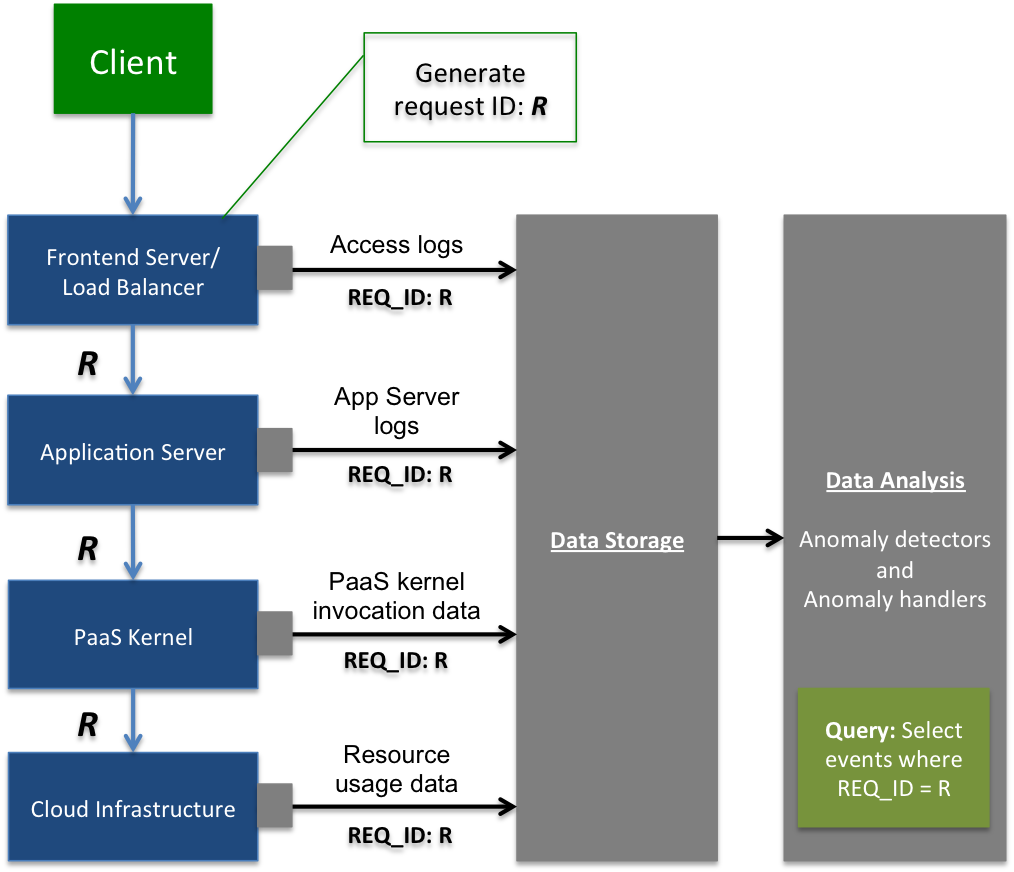
\includegraphics[scale=0.5]{apm_architecture}
\caption{Roots APM architecture.  Roots injects a request ID ($R$) at request
ingress that it uses to correlate events at each level of the stack.}
\label{fig:apm_architecture}
\end{figure}
%
%Figure~\ref{fig:apm_architecture} illustrates the high-level architecture of Roots, and how 
%it fits into the PaaS stack. APM components are shown in grey, with their interactions indicated
%by the black lines. The small grey boxes attached to the PaaS components represent the
%agents used to instrument the cloud platform for data collection purposes. 
%In the diagram a user request is getting tagged with the identifier value
%$R$ at the front-end server. This identifier is passed down to the lower layers of the cloud
%along with the request. Events that occur in the lower layers as a result of processing this request
%are recorded with the request identifier $R$, so we can correlate them later. For example, in the 
%data analysis component we can run a filter query to select all the events related to a particular
%request (as shown in the pseudo query in the diagram). Or we can run a ``group by'' 
%query to select all events, and aggregate them by the request identifier.

Figure~\ref{fig:apm_architecture} shows Roots collecting data from all
layers in a PaaS stack (i.e. full stack monitoring). 
%From the front-end server layer we gather information related to incoming application
%requests. A big part of this is scraping the HTTP server access logs, which indicate request timestamps,
%source and destination addressing information, response time (latency) and other HTTP message
%parameters. This information is readily available for harvesting in most technologies used as front-end
%servers (e.g. Apache HTTPD, Nginx). Additionally we may also collect information pertaining to active
%connections, invalid access attempts and other errors.
%
%From the application server layer we collect basic application logs as well as any other
%metrics that can be easily collected from the application runtime. This may include some process level
%metrics indicating the resource usage of the individual application instances. Additionally, Roots
%employs a set of per-application benchmarking processes that periodically probes 
%different applications
%to measure their performance. These are lightweight, stateless processes managed by the Roots framework.
%Data collected by these processes will also be sent to data storage component, and will be available
%for analysis as per-application time series data. 
%
%In particular, for each request 
%at the PaaS kernel layer we collect information regarding all kernel invocations
%made by the applications. This requires intercepting the PaaS kernel invocations
%at runtime. This must be done carefully as to not introduce a noticeable
%overhead to the application execution. For each PaaS kernel invocation, 
%we can capture the 
%following parameters.
%\begin{itemize}
%\item Source application making the kernel invocation
%\item Timestamp
%\item A sequence number indicating the order of PaaS kernel invocations within an application request
%\item Target kernel service and operation
%\item Execution time of the invocation
%\item Request size, hash and other parameters
%\end{itemize}
Collecting this information along with the request identifiers generated by the
front-end server
enables tracing the execution of application requests through the cloud platform. In addition
to the data collecting agents directly integrated with the cloud platform, Roots employs
a collection of application benchmarking processes that periodically measures
application latency. The measurements taken by these processes are mainly used to
evaluate the performance SLOs of each application.

%Finally, at the lowest infrastructure level, we can collect information related to virtual machines, containers
%and their resource usage. We can also gather metrics on network usage by individual components which
%might be useful in a number of traffic engineering use cases. Where appropriate we can also scrape
%hypervisor and container manager logs to get an idea of how resources are allocated and released over
%time.

To avoid introducing delays to the application request processing flow, we implement
all Roots data collecting agents as asynchronous tasks. That is, none of them would
suspend application request processing to report data to the data storage components.
We make sure that all expensive I/O tasks related to data collection and storage are
executed out of the request processing flow.
In particular, all data is collected into log files or memory buffers that are local to the components being
monitored. This locally collected (or buffered) data is periodically sent
to the data storage components of Roots using separate background tasks and batch communication
operations. Also special care is taken to isolate the activities in the cloud from potential
failures in the Roots data collection or storage components.

\subsubsection{Data Storage}

The Roots data storage is a database that supports persistently storing monitoring data, and running
queries on them.  
%Cloud providers have the freedom to implement this component in any way they see fit, as long
%as it scales to the number of applications deployed in the cloud platform. 
Most data retrieval queries executed
by Roots use application and time intervals as indices. Therefore a database that can index monitoring
data by application, and then organize records by timestamp will greatly improve the query performance.
It is also acceptable to remove old monitoring data to make room for more recent events, since Roots
is performing anomaly detection using the most recent data in near real time.

\subsubsection{Data Analysis}

Roots data analysis component uses two basic abstractions: \textit{anomaly detectors} 
and \textit{anomaly handlers}.
Anomaly detectors are processes that periodically analyze the data collected for
each deployed application. Roots supports multiple detector implementations, where each implementation
uses a different statistical method to look for performance anomalies. Detectors are configured
per-application, making it possible for different applications to use different anomaly 
detectors. Roots also supports multiple concurrent anomaly detectors on the same application, which can be used
to evaluate the efficiency of different detection strategies for any given application. Each
anomaly detector has an execution schedule (e.g. run every 60 seconds), and a sliding window 
(e.g. from 10 minutes ago to now)
associated with it. The boundaries of the window determines the time range
of the data processed by the detector at any round of execution. Window is updated 
after each round of execution. 
%Our anomaly detector abstraction is general
%enough to support detecting a wide range of anomalies. However, in our work we
%mainly focus on anomaly detectors that check for violations of performance SLOs.

When an anomaly detector finds an anomaly in application performance, it sends an event
to a collection of anomaly handlers. The event encapsulates a unique anomaly identifier, 
timestamp, application identifier and the source detector's sliding window that correspond to the
anomaly. Anomaly handlers are configured globally (i.e. each handler
receives events from all detectors), but each handler can be programmed to handle only
certain types of events. Furthermore, they can fire their own events, which are also delivered to
all the listening anomaly handlers. Similar to detectors, Roots supports multiple anomaly handler
implementations -- one for logging anomalies, one for sending alert emails, one
for updating a dashboard etc. 

Additionally, Roots includes two special anomaly handler
implementations: a workload change analyzer, and a bottleneck identifier.
The communication between detectors and handlers can be efficiently implemented
using shared memory as explained in section ~\ref{sec:process_mgt}.

%The ability of anomaly handlers to fire their own events, coupled with their support
%for responding to a filtered subset of incoming events enables constructing
%elaborate event flows with sophisticated logic. For example, the workload
%change analyzer can run some analysis upon receiving an anomaly event
%from any anomaly detector. If an anomaly cannot be associated with a workload
%change, it can fire a different type of event. The bottleneck identifier, can
%be programmed to only execute its analysis upon receiving this second type of event.
%This way we perform the workload change analysis first, and perform the
%systemwide bottleneck identification only when it is required to do so.

%Both the anomaly detectors and anomaly handlers work with fixed-sized sliding windows.
%They can discard any old data as the sliding window moves along the time line.
%Therefore the amount of state information these entities must keep in memory has
%a strict upper bound. 
%The extensibility of Roots is primarily achieved through the abstractions of anomaly
%detectors and handlers. Roots makes it simple to implement new detectors and handlers,
%and plug them into the system. Both the detectors and the handlers are executed
%as lightweight processes that do not interfere with the rest of the processes in
%the cloud platform. Failures in detectors and handlers have no impact
%on the cloud platform or the deployed applications.

\subsubsection{Roots Pods}
\label{sec:process_mgt}

%\begin{figure}
%\centering
%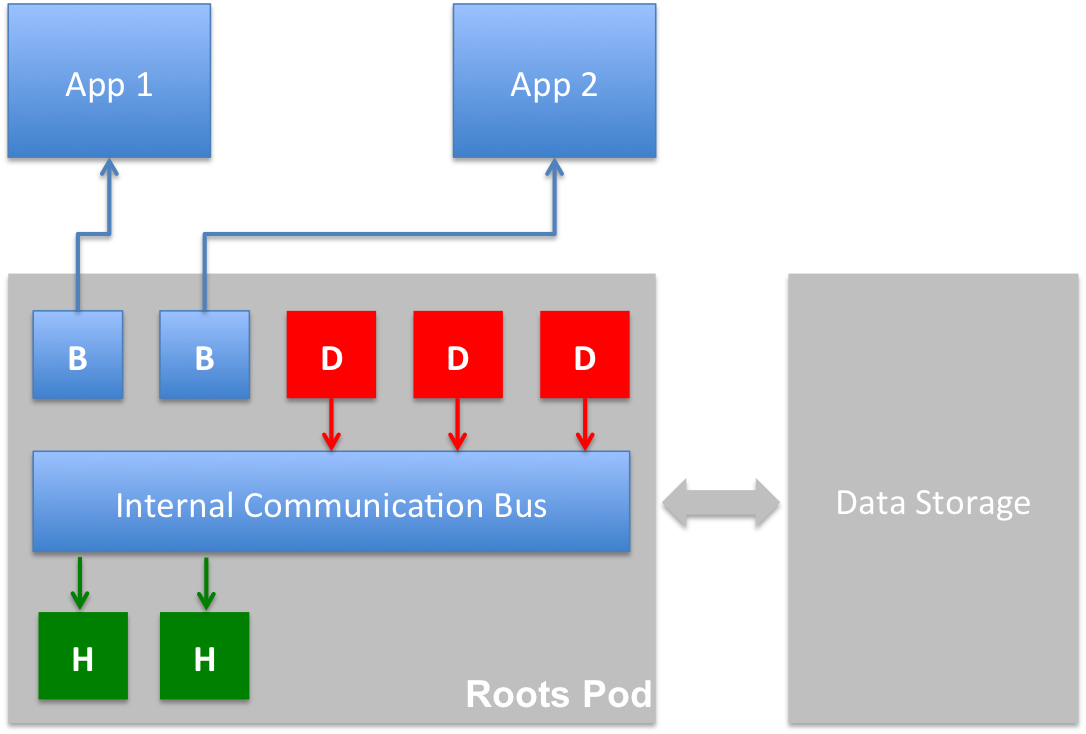
\includegraphics[scale=0.45]{roots_pod}
%\caption{Anatomy of a Roots pod. The diagram shows 2 application benchmarking processes (B), 
%3 anomaly detectors (D), and 2 handlers (H). Processes communicate via a shared
%memory communication bus local to the pod.}
%\label{fig:roots_pod}
%\end{figure}
%Most data collection activities in Roots can be treated as passive -- i.e. they
%happen automatically as the applications receive and process requests in the cloud
%platform. They do not require explicit scheduling or management. In contrast,
%application benchmarking and data analysis are active processes that require
%explicit scheduling and management.  This is achieved by 

Roots groups data analysis processes (i.e. anomaly detectors and handlers), 
and application benchmarking processes into units called \textit{Roots pods}. 
Each Roots pod is responsible for starting and maintaining a collection of
benchmarkers and data analysis processes. 
Each of these processes are light enough, so as to pack a large number of them
into a single pod. Pods are self-contained entities, and there is no inter-communication
between pods. 
Processes within a pod can efficiently communicate with each other 
using shared memory, and call out to the central Roots data storage to retrieve 
collected performance data for analysis. This enables starting and stopping 
Roots pods with minimal impact on the overall monitoring system. Furthermore, pods
can be replicated for high availability, and application load can be distributed
among multiple pods for scalability.

%Figure~\ref{fig:roots_pod} illustrates a Roots pod monitoring two applications.
%It consists of two benchmarking processes, three anomaly detectors and 
%two anomaly handlers. The anomaly detectors and handlers communicate
%using an internal shared memory communication bus, so that events triggered by one anomaly
%detector flow into all handlers. 

%To automate the process of managing pods, they can be tied into the core
%process management framework of the PaaS cloud. That way whenever the cloud
%platform initializes, a collection of pods can be started automatically.
%Application deployment process of the PaaS cloud can be augmented
%to register each new application with one of the available pods, so that the
%benchmarkers and anomaly detectors can start running on the application.
%Moreover, pods can be moved around or restarted as needed in response
%to errors and autoscaling events that occur in the cloud platform.

%\section{Survey on Google App Engine Applications}
%\label{sec:survey}
We start by statically analyzing a random sample of cloud applications to learn various properties related
to branching, looping and usage of cloud SDK interfaces in the applications written for PaaS environments. 
We scour the GitHub source code repository for open source Google App Engine applications written in Java,
and randomly select a population of 35 applications. These applications are subjected to a thorough analysis
using the Soot framework to study their code patterns. Our analysis detected 1458 different methods in all the
applications. In this section we present a detailed overview of the observations made in this study. We note that
our design and implementation of Cerebro, and the associated experiments have been influenced by 
these observations in several ways.

\begin{figure}
\centering
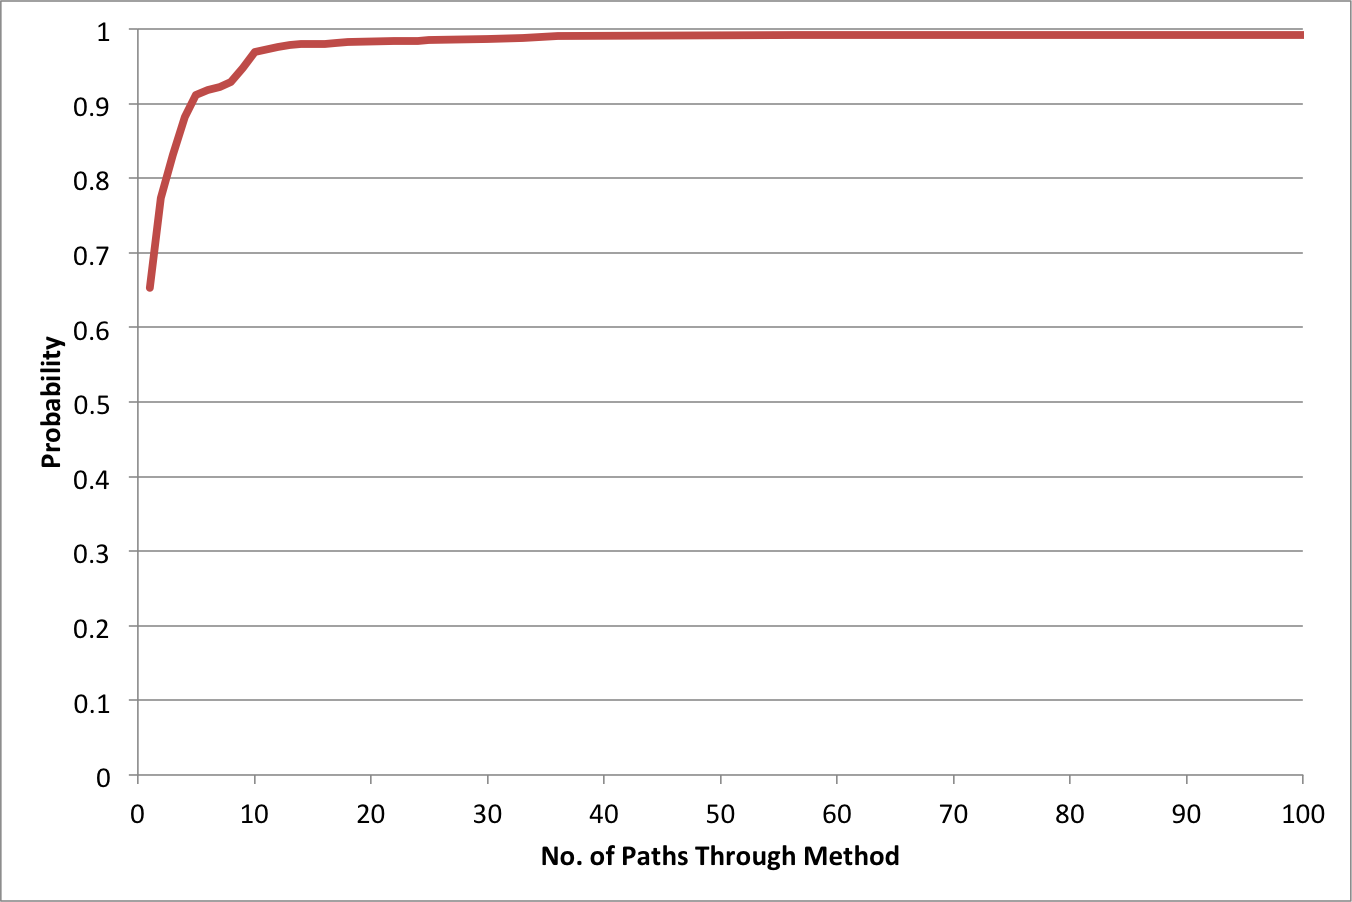
\includegraphics[scale=0.35]{path_count_cdf}
\caption{CDF of path counts through methods in web applications.}
\label{fig:path_count_cdf}
\end{figure}

FIgure~\ref{fig:path_count_cdf} shows the number of paths through methods, and the probability of encountering
a method with a given number of paths (in other words the branching behavior of methods). According to this CDF, 
around 97\% of the methods considered in the analysis have 10 or less paths going through them. About 99\% of 
the methods have 36 or less paths going through them. However, this CDF does have a very long tail, going all the way
up to 34992 (not shown in the figure -- the x-axis of the CDF has been truncated at 100 paths). Still, it is interesting to note that more
than half the methods considered in the analysis, 65\% to be precise, have no more than exactly 1 path (i.e. no branches).
This implies that roughly 65\% of the time, Cerebro has to only generate a single sequence of predictions. In cases
where there are multiple branches, Cerebro's unique path detection mechanism can help significantly 
reduce the number of prediction traces that need to be generated.

Next we look at the looping behavior of the 35 web applications used in the study. As it turns out 1286 of the methods (88\%)
considered in the study
do not have any loops. Only 172 methods (12\%) consist of loops. Clearly the PaaS SDK and the associated coding restrictions
are making loops a somewhat rare feature in the cloud applications. A large majority of the loops (61\%) encountered in our analysis are
preceded by a call to a batch read operation in the datastore cloud SDK of Google App Engine. The purpose of these loops is to simply iterate
through the results returned by the read. We use this vital piece of information when designing the loop handling capability of
Cerebro. Whenever Cerebro encounters a loop, it checks whether the loop is preceded by a batch read to the datastore. Watchtower
benchmarks this code pattern (batch read followed by a loop), so that Cerebro can use the gathered measurements to make
more accurate predictions regarding loops.

\begin{figure}
\centering
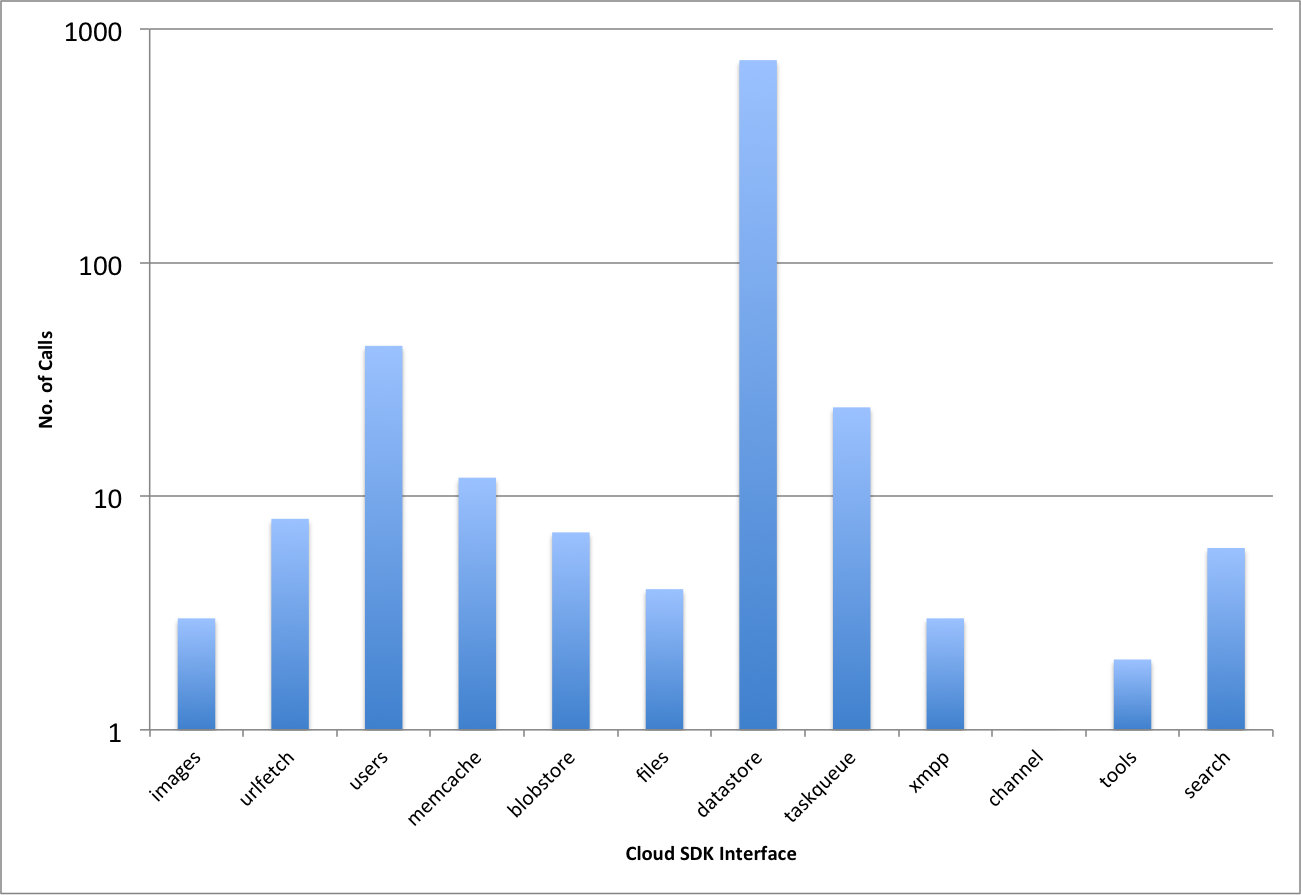
\includegraphics[scale=0.35]{sdk_call_counts}
\caption{Number of times different cloud SDK interfaces are called in web applications.}
\label{fig:sdk_call_counts}
\end{figure}

Figure~\ref{fig:sdk_call_counts} illustrates the number of times each cloud SDK interface has been called in the sample of
35 web applications. Clearly datastore is the most commonly used interface as far as Google App Engine applications are 
concerned. This is because data storage and access is a fundamental capability required by most web applications. 
Some of the other widely used interfaces include users, taskqueue and memcache. 

\begin{figure}
\centering
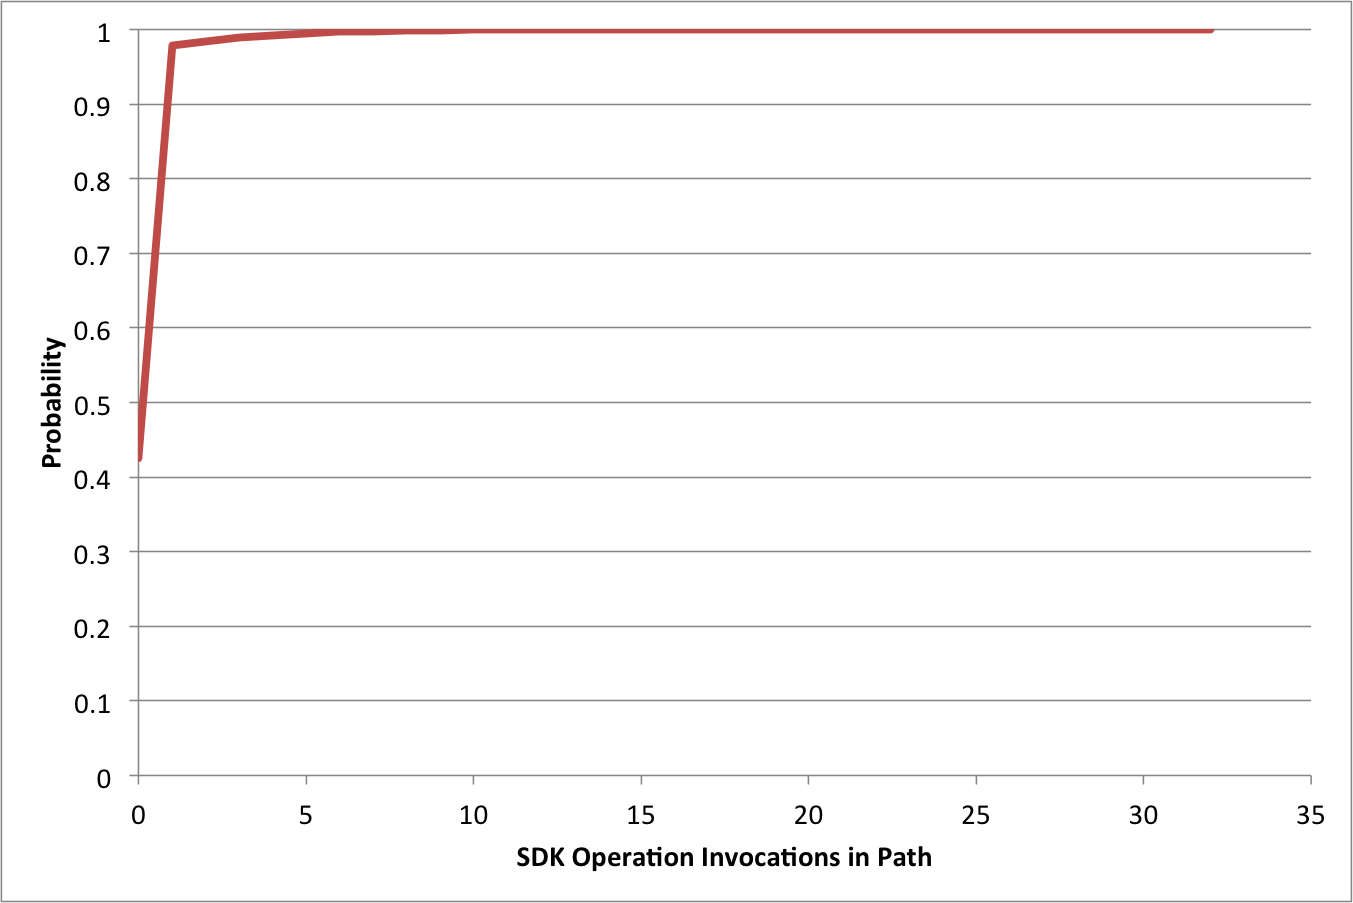
\includegraphics[scale=0.35]{sdk_call_count_cdf}
\caption{CDF of cloud SDK call counts in web applications.}
\label{fig:sdk_call_count_cdf}
\end{figure}

Finally we explore the number of cloud SDK calls made in different paths of execution in the web applications. For this study
we consider all the paths of execution through the methods. This amounted to 64780 total paths. Figure~\ref{fig:sdk_call_count_cdf}
shows the number of cloud SDK calls in the paths, and the probability of finding a path with a given number of cloud SDK calls.
According to that around 98\% of the paths have 1 or less cloud SDK call. The probability of finding an execution path with more than
5 cloud SDK calls is smaller than 0.01. This implies in most cases Cerebro will make response time predictions without having to 
aggregate multiple time series together.

\vspace{-0.10in}
\section{Cerebro}
\label{sec:design}
%Given the restricted execution domain of PaaS clouds, we believe that it is possible
to design a system that predicts response time SLAs for PaaS-hosted web APIs using only
static information from the web API code itself.  To enable this, we design Cerebro
with three primary components:
\begin{itemize}
\item A static analysis tool that extracts sequences of cloud SDK operations for 
each path through a method (web API operation),
\item A monitoring agent that runs in the target PaaS and efficiently monitors 
the performance of the underlying cloud SDK operations (which we will call Watchtower), and
\item A prediction mechanism that uses the outputs of these two components to accurately predict an upper bound on the execution time of the web API (which we call the SLA predictor).
\end{itemize}
In our prototype, we invoke Cerebro each time a 
web API is deployed.
%when a developer uploads their application to the cloud platform, Cerebro performs
%the static analysis on the web API and requests a prediction for the longest path (currently
%number and type of SDK operations) for each web API operation from the SLA predictor.
%The SLA predictor accesses the time series data from Watchtower to produce an 
%SLA prediction for each operation.

%\begin{figure}
%\centering
%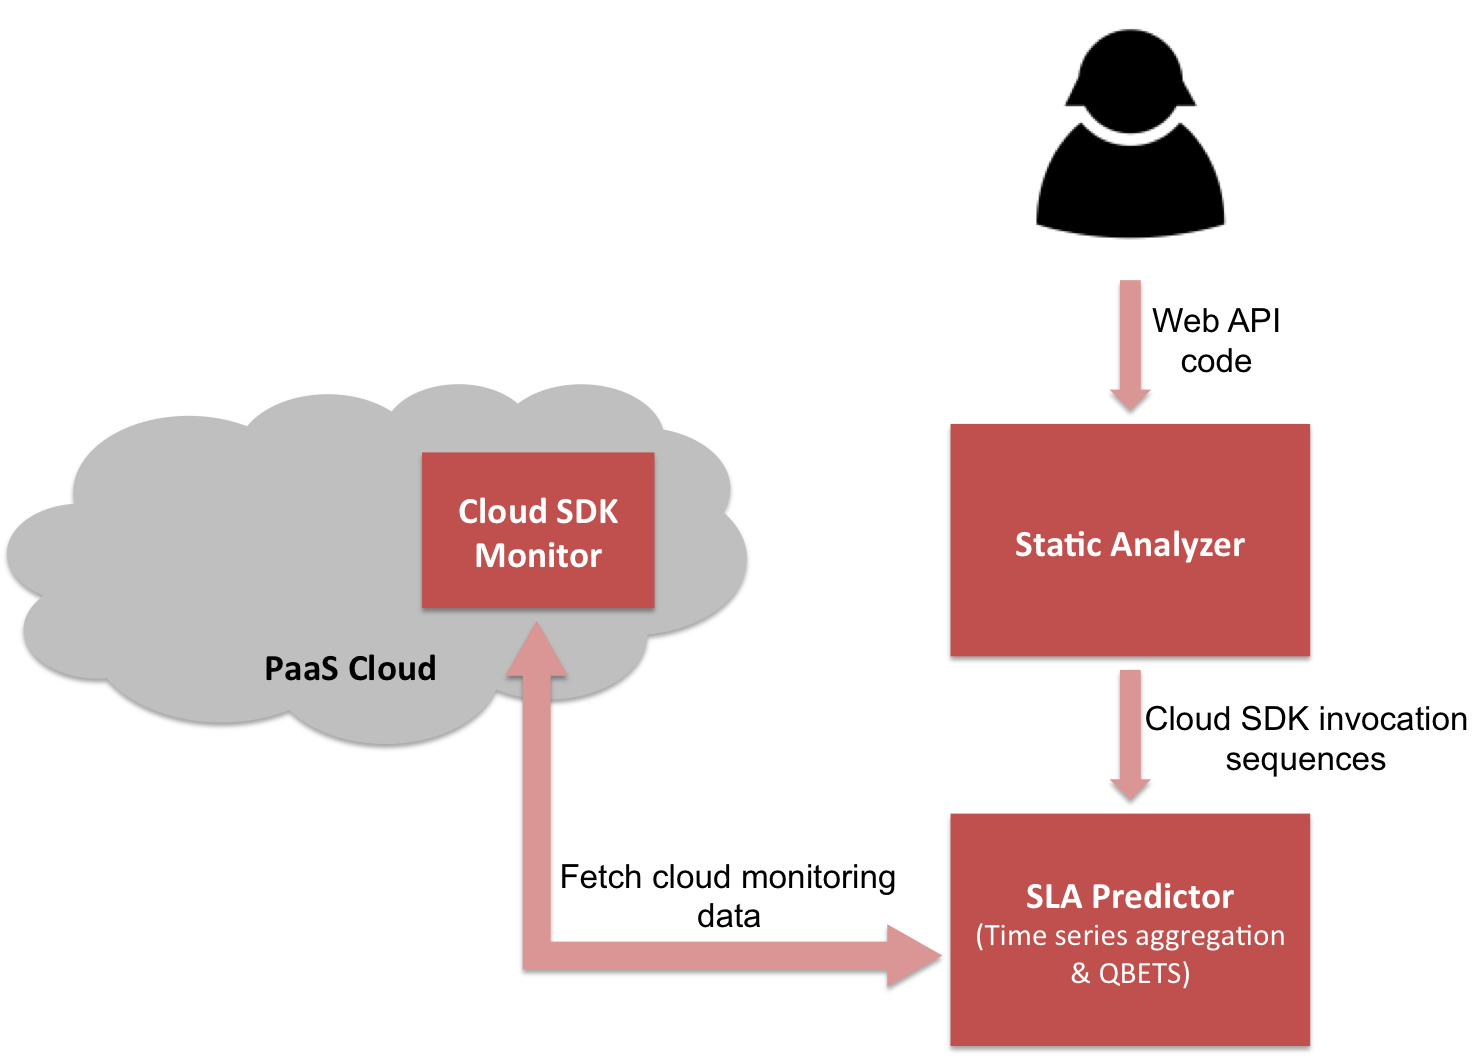
\includegraphics[scale=0.35]{cerebro_arch}
%\caption{Cerebro architecture and component interactions.}
%\label{fig:cerebro_arch}
%\end{figure}

%Additionally, we need a component that combines the results generated by above two components
%to make SLA predictions. Figure~\ref{fig:cerebro_arch} shows an overview of the resulting architecture.

\subsection{Static Analysis}
 This component analyzes the source code 
(or some intermediate representation of it), to identify
 the cloud SDK operations invoked by a given web API code. 
Since a web API code can only make a finite
 number of cloud SDK invocations, and since PaaS clouds only support a finite number of cloud
 SDK operations, it is possible to design an algorithm that
 extracts all cloud SDK invocations from any given web API code. 

Cerebro performs a simple construction and interprocedural static analysis 
of a method's control flow graph 
(CFG)~\cite{Allen:1970:CFA:800028.808479,Aho:1986:CPT:6448,Morgan:1998:BOC:288765,Muchnick:1998:ACD:286076} for each API method (externally facing) in a web API. 
The algorithm extracts all cloud SDK operations along
each path through the method.  Cerebro analyzes calls to other web API functions
that the method calls, recursively.  Cerebro caches cloud SDK details for each function 
once analyzed so that it can be reused efficiently for other call sites to the same
function. Cerebro does not analyze third-party library calls, if any.  Cerebro encodes
each cloud SDK call sequence for each path in a lookup table. Cloud SDK calls are 
easily identified by name, similarly to library calls.

To handle loops, we first extract them from the CFG and 
annotate any cloud SDK invocations that occur within them, in the cloud SDK sequence
for the path.  We annotate each with an estimate on the number of times
the loop is likely to execute in the worst case. We use a simple static
loop bounds estimator 
based on past work~\cite{bygde2010static,Gulwani:2009:CRP:1542476.1542518,Lokuciejewski:2009:FPS:1545006.1545064,Hunt:2006:PCL:1167999.1168026}
to enable this.  We perform cloud SDK operation annotation during CFG analysis
and estimate loop bounds separately afterward.

We have found (and show in our characterization of App Engine web APIs in the previous
section) that loops in these programs are rare and when they do occur, they are
used to iterate over a particular data set, commonly returned from the database.
For such data dependent loops, we estimate the bounds if specified 
in the cloud SDK call (e.g. the maximum number of 
entities to return~\cite{gae-fetch-options}).
If our analysis is unable to estimate the bounds for these loops, the tool asks
the developer for an estimate of the likely data set size.

\subsection{Platform Monitoring Agent: Watchtower}
Watchtower is the Cerebro component that tracks the performance of individual
cloud SDK operations within a PaaS system.  It is possible to implement
Watchtower as an integrated PaaS service or as a PaaS application (web API).
Watchtower runs in the background with but separate from other PaaS-hosted web APIs.
It performs cloud SDK operations on synthetic datasets and records timestamped response
times in the PaaS datastore on a operation basis.  Watchtower includes
benchmarks for loop iteration over datastore numbers of entities 
(i.e. iterative datastore reads)
that some App Engine web APIs employ.  
Watchtower periodically garbage collects old records to eliminate unnecessary storage.

The frequency with which
Watchtower collects data determines how often Cerebro 
is able to make SLA predictions for web APIs. Currently, we use a period of one minute
but this value is configurable.  Cerebro benchmarks iteratvie datastore reads
using 1, 1000, and 1000000 entities.  Cerebro monitoring is straightforward and
benchmarks can easily be added and customized to capture common PaaS-hosted web API
patterns.


\subsection{Making SLA Predictions}

To make SLA predictions, Cerebro uses 
Queue Bounds Estimation from Time Series (QBETS)~\cite{Nurmi:2007:QQB:1791551.1791556},
a non-parametric time series analysis method that we developed in prior work.
We originally designed QBETS for
predicting the scheduling delays for the batch queue systems 
used in high performance computing environments. 
We adapt it for use ``as-a-service'' in PaaS systems 
to predict the execution time of web APIs.

A QBETS analysis requires three inputs:
\begin{enumerate}
\item A time series of data generated by a continuous experiment,
\item The percentile for which an upper bound should be predicted ($p \in [1..99]$)
\item The upper confidence level of the prediction ($c \in (0,1)$)
\end{enumerate}

QBETS uses this information to predict an upper bound for 
the $p$-th percentile of the time series.
The predicted value has a probability of $0.01p$ of 
being greater than or equal to the next data point that
will be added to the time series by the continuous experiment. 
The upper confidence level $c$ serves as a conservative
bound on the predictions. That is, predictions made with an upper confidence 
level of $c$ will overestimate
the true percentile with a probability of $1-c$. This confidence guarantee 
is necessary because 
QBETS does not determine the 
percentiles of the time series precisely, but only estimates them. 

To further clarify what QBETS does, assume a continuous experiment 
that periodically measures the
response time of a web API. This results in a time series of 
response time data. Suppose at time $t$,
we run QBETS on the time series data collected so far 
with $p=95$ and $c=0.01$. The prediction returned
by QBETS has a 95\% chance of being greater than or equal 
to the next response time value measured
by our experiment after time $t$. Since $c=0.01$, the predicted value has a 99\% chance of
overestimating the true 95th percentile of the time series.

We find QBETS to be an ideal fit for our work due to several reasons. 
\begin{itemize}
\item QBETS works with time series data. Since
cloud SDK benchmarking data can be easily represented as time series,
they are highly amenable for QBETS analysis. 
\item QBETS makes predictions regarding the
future outcomes of an experiment by looking at the past 
outcomes -- an idea that aligns with our
goal of predicting future API response times from past cloud SDK benchmarking data. 
\item Response time
SLAs of web APIs should be specified with exact correctness 
probabilities and confidence levels for
them to be useful to developers and PaaS administrators. QBETS meets these requirements.
\item QBETS is 
simple, efficient and has been applied successfully to analyze a wide range of time series 
data, including correlated and uncorrelated data, in the past.
\end{itemize}

We now describe the Cerebro process.
Recall that our static analysis produces a list of annotated cloud SDK invocation sequences.
We start by pruning this list to eliminate duplicates. 
Duplicates occur when a web API code has
multiple paths of execution, where more than one path consists of the same sequence of cloud 
SDK invocations. Then for each sequence of cloud SDK 
invocations present in the pruned list, we
perform the following operations:

\begin{enumerate}
\item Retrieve benchmarking data from Watchtower 
for all operations in the sequence. Watchtower provides
this information as ordered time series data (one time series per cloud SDK operation).
\item Align all retrieved time series across operations and aggregate
to form a single time series for the sequence of cloud SDK operations.
\item Pass the aggregate time series to QBETS along with the 
desired $p$ and $c$ values to predict an
upper bound. 
\end{enumerate}

This process is exemplified as follows.
Suppose our static analysis results in the
cloud SDK invocation sequence $<op_{1},op_{2},op_{3}>$. 
Lets assume Watchtower has the following
time series data collected for the three operations in the sequence.

\begin{itemize}
\item $op_{1}$: $[t_{0}: 5, t_{1}: 4, t_{2}: 6, ...., t_{n}: 5]$
\item $op_{1}$: $[t_{0}: 22, t_{1}: 20, t_{2}: 21, ...., t_{n}: 21]$
\item $op_{1}$: $[t_{0}: 7, t_{1}: 7, t_{2}: 8, ...., t_{n}: 7]$
\end{itemize}

Here $t_{m}$ are timestamp values Watchtower has assigned to 
each data point. We align the three
time series, so that values with the same timestamp line up 
together, and aggregate the results
to obtain the following time series.

$[t_{0}: 34, t_{1}: 31, t_{2}: 35, ...., t_{n}: 33]$

Then we pass the aggregate time series to QBETS for analysis, and
treat the QBETS prediction as an SLA for the web API code.
If the QBETS predicted value is $Q$ milliseconds, 
we can form the SLA as ``the web API responds 
under $Q$ milliseconds, $p$ percent of the time''. 
When the code has multiple paths of execution (and
hence multiple sequences of cloud SDK operations), 
we predict more than one SLA for the API. In
such cases we treat the SLA with highest predicted value 
as the final SLA (i.e. the worst case SLA).

When the static analysis produces cloud SDK invocation 
sequences with information about loops, Cerebro performs an additional step.
If some operation has been tagged as being inside a loop, where the loop
bounds have been estimated, the time series data corresponding to that 
operation should be multiplied 
by the loop bound estimate, before aggregating. In cases where the operation 
is inside a data dependent loop, we request the time series data from a 
Watchtower iterative datastore read benchmark for a number of entities 
equal to or larger than the annotation. 

Another characteristic of QBETS is its warm up period.
QBETS requires a sufficiently large number of data points
in the input time series before it can make an accurate prediction. 
Specifically, we have proved that QBETS must to see 
at least $log(c)/log(0.01p)$ data points
before it can start making reliable predictions. 
This means, if we are interested in predicting the 95th percentile
of the API execution time, with an upper confidence of 0.01, 
Cerebro must feed QBETS with a time series that
contains at least 90 data points. We use this information to control 
Watchtower garbage collection.

\subsection{Cerebro Workflow}

%\begin{figure}
%\centering
%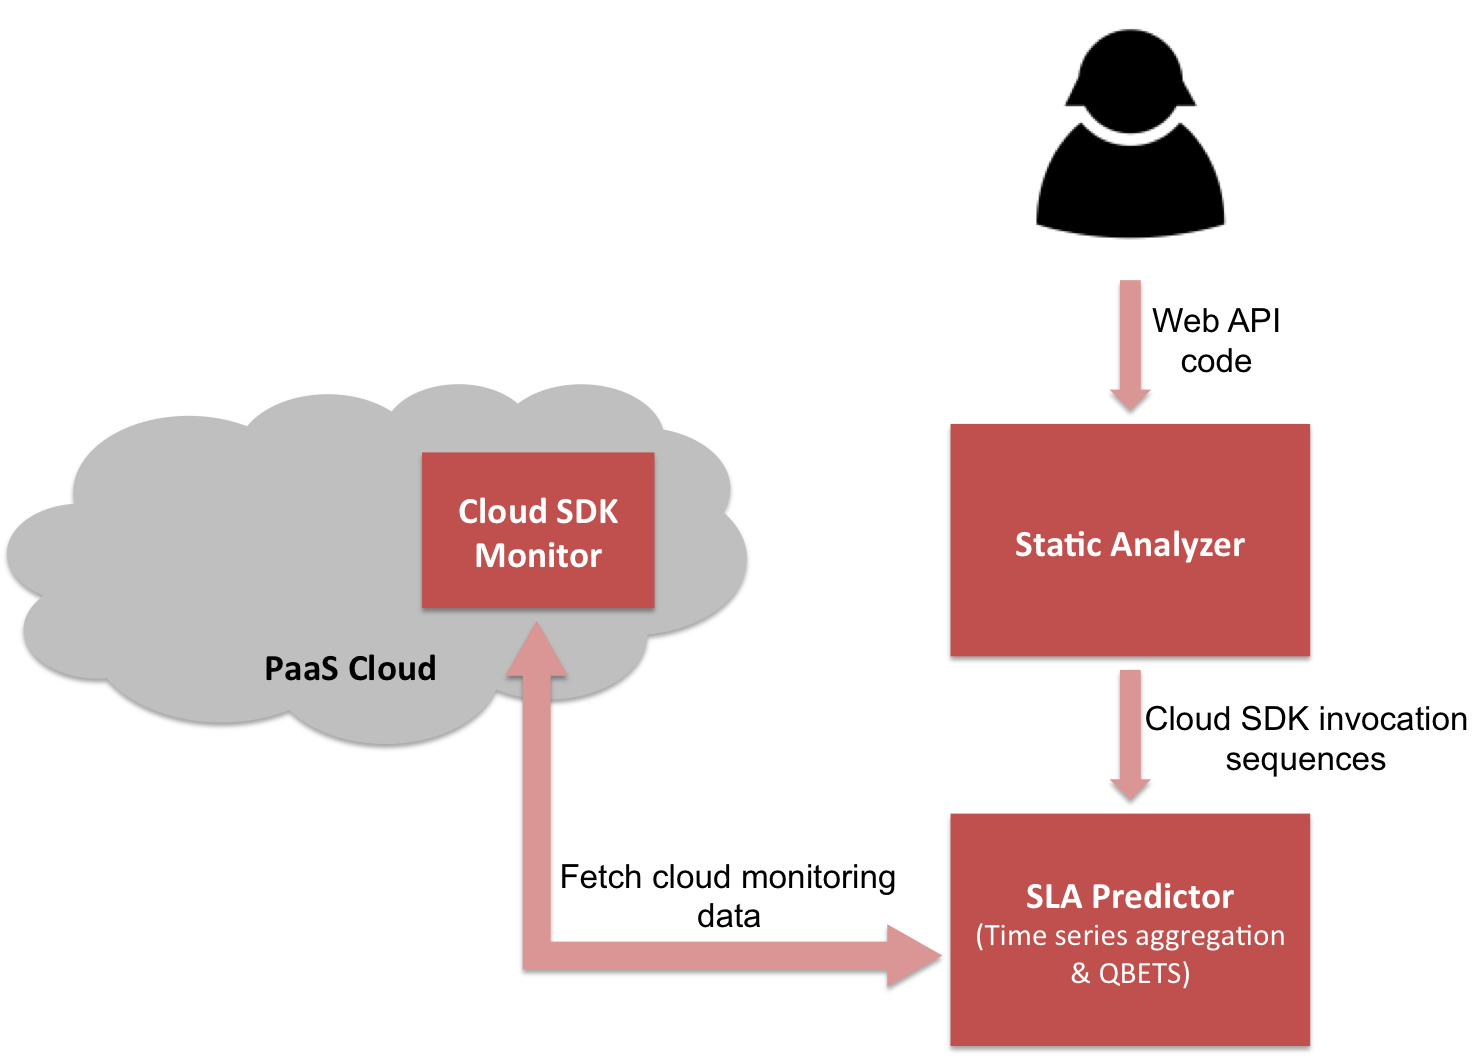
\includegraphics[scale=0.35]{cerebro_arch}
%\caption{Cerebro architecture and component interactions.}
%\label{fig:cerebro_arch}
%\end{figure}

Although we invoke Cerebro as part of the web API deployment process. Developers
can also do so during development using Cerebro's static analysis tool and interacting
with the Cerebro service in a PaaS cloud.
The static analyzer extracts the sequences of cloud SDK invocations from 
the web API code and passes them to Cerebro.
Cerebro contacts Watchtower 
to retrieve the relevant cloud SDK operation
benchmark data (time series) and aggregates them for QBETS processing.
Cerebro then generates a prediction using its QBETS service, which returns a prediction
for the percentile ($p$) and the upper confidence ($c$) values of interest.

The predictions can be used in many ways. In the simplest case they can be
used to clearly document the API SLAs, so that API consumers can stay informed about what 
type of performance to expect from the APIs they use. In a somewhat advanced context, 
Cerebro predictions can guide the API developers on how to program web APIs 
to support highly competitive SLAs. In an
more sophisticated environment, the Cerebro predictions can be used to 
enforce SLA-related policies on web APIs deployed in the cloud. Such an implementation
can run Cerebro on web APIs as they are submitted for deployment, 
and reject any APIs that do not
support the desired performance level.

Given the restricted application domain of PaaS-hosted web APIs, we believe
that it is possible to design a system that predicts response time SLAs for
them using only static information from the web API code itself.  To enable
this, we design Cerebro with three primary components:
\begin{itemize}
\item A static analysis tool that extracts sequences of cloud SDK operations for 
each path through a method (web API operation),
\item A monitoring agent that runs in the target PaaS, and efficiently monitors 
the performance of the underlying cloud SDK operations, and
\item A prediction mechanism that uses the outputs of these two components to accurately predict an upper bound on the execution time of the web API.
\end{itemize}
We overview each of these components in the subsections that follow and then 
present the Cerebro workflow with an example.

\subsection{Static Analysis}
 This component analyzes the source code of the web API
(or some intermediate representation of it) and extracts a sequence of cloud API operations.
We implement our analysis for Java bytecode programs
using the Soot framework~\cite{Vallee-Rai:2010:SJB:1925805.1925818}.
Currently, our prototype analyzer considers the 
following Java codes as exposed web APIs.
\begin{itemize}
\item classes that extend the \textit{javax.servlet.HttpServlet} class (i.e. Java servlet implementations)
\item classes that contain JAXRS \textit{@Path} annotations, and
\item any other classes explicitly specified by the developer in a special configuration file.
\end{itemize}

Cerebro performs a simple construction and inter-procedural static analysis 
of control flow graph 
(CFG)~\cite{Allen:1970:CFA:800028.808479,Aho:1986:CPT:6448,Morgan:1998:BOC:288765,Muchnick:1998:ACD:286076} for each web API operation.
The algorithm extracts all cloud SDK operations along
each path through the methods. Cerebro analyzes calls to other functions
that the method calls, recursively.  Cerebro caches cloud SDK details for each function 
once analyzed so that it can be reused efficiently for other call sites to the same
function. Cerebro does not analyze third-party library calls, if any 
(which in our experience typically do not contain cloud SDK calls). Cerebro encodes
each cloud SDK call sequence for each path in a lookup table. We identify
cloud SDK calls by their Java package name (e.g. \texttt{com.google.appengine.apis}).

To handle loops, we first extract them from the CFG and 
annotate all cloud SDK invocations that occur within them.
We annotate each such SDK invocation with an estimate on the number of times
the loop is likely to execute in the worst case. 
We estimate loop bounds using a loop bound prediction algorithm 
based on abstract interpretation~\cite{bygde2010static}. 

As shown in the previous section, loops in these programs 
are rare and, when they do occur, they are
used to iterate over a data set returned from a database.
For such data dependent loops, we estimate the bounds if specified 
in the cloud SDK call (e.g. the maximum number of 
entities to return~\cite{gae-fetch-options}).
If our analysis is unable to estimate the bounds for these loops, Cerebro prompts
the developer for an estimate of the likely data set size and/or loop bounds.

\subsection{PaaS Monitoring Agent}
Cerebro monitors and records the response time of individual
cloud SDK operations within a running PaaS system.  Such support can be 
implemented as a PaaS-native feature or as
a PaaS application (web API); we use the latter in our prototype.
The monitoring agent runs in the background with, but separate from, 
other PaaS-hosted web APIs.
The agent invokes cloud SDK operations periodically on synthetic data sets and 
records timestamped response times in the PaaS datastore for each cloud SDK
operation.
Finally, the agent periodically reclaims old measurement data
to eliminate unnecessary storage. The Cerebro monitoring and reclamation 
rates are configurable and monitoring benchmarks can be added and customized
easily to capture common PaaS-hosted web API coding patterns.

In our prototype, the agent monitors the datastore and memcache services
every 60 seconds. In addition, it 
benchmarks loop iteration over datastore entities to capture
the performance of iterative datastore reads for datastore result set sizes 
of 10, 100, and 1000. We limit ourselves to these values because the PaaS requires
that all operations complete (respond) within 60 seconds -- so the data
sizes returned are typically small.

\subsection{Making SLA Predictions}
\label{sec:qbets}
To make SLA predictions, Cerebro uses 
Queue Bounds Estimation from Time Series (QBETS)~\cite{Nurmi:2007:QQB:1791551.1791556},
a non-parametric time series analysis method that we developed in prior work.
We originally designed QBETS for
predicting the scheduling delays for the batch queue systems 
used in high performance computing environments but it has proved effective
in other settings where forecasts from arbitrary times series are
needed~\cite{uptime-bootstrap,quant-est,euca-power-tr-14}.  In 
particular, it is both
non-parametric and it automatically
adapts to changes in the underlying time series dynamics making it useful in
settings where forecasts are required from arbitrary data with widely varying
characteristics. 
%We adapt it herein for use ``as-a-service'' in PaaS systems 
%to predict the execution time of web APIs.

A QBETS analysis requires three inputs:
\begin{enumerate}
\item A time series of data generated by a continuous experiment.
\item The percentile for which an upper bound should be predicted ($p \in [1..99]$).
\item The upper confidence level of the prediction ($c \in (0,1)$).
\end{enumerate}

QBETS uses this information to predict an upper bound for 
the $p^{th}$ percentile of the time series.  It does so by treating each
observation as a Bernoulli trial with probability $0.01p$ of succeess.  Let $q
= 0.01p$.  If there are $n$ observations, the probability of there being
exactly $k$ successes is described by a Binomial distribution (assuming
observation independence)
having parameters $n$ and $q$.  If $Q$ is the $p^{th}$ percentile of the
distribution from which the observations have been drawn, the equation 
\vspace{-0.1in}
\begin{equation}\label{sumformula}
1 - \sum_{j=0}^k { n \choose j } \cdot (1-q)^{j} \cdot q^{n-j}
\end{equation}
gives the probability that more than $k$ obervations are greater than $Q$.
As a result, the $k^{th}$ largest value in a sorted list of $n$ observations
gives an upper $c$ confidence bound on $Q$ when $k$ is the smallest integer
value for which Equation~\ref{sumformula} is larger than $c$.

More succinctly, QBETS sorts the observations in a history of observations,
and computes the value of $k$ that constitutes an index into 
this sorted list of the observation that is the upper $c$ confidence bound on
the $p^{th}$ percentile. The methodology assumes that the time series of 
observations is 
ergodic so that, in the long run, the confidence bounds are accurate.  

QBETS also attempts to detect change points in the time series of observations 
so that it can apply this inference technique to only the most recent 
segment of the series that appears to be stationary.  
To do so, it compares
percentile bounds predictions with observations throughout the series and
determines where thes series is likely to have undergone a change.  It then
discards observations from the series prior to this change point and
continues.  As a result, when QBETS starts, it must ``learn'' the series by
scanning it in time series order to determine the change points.  We report
Cerebro learning time in our empirical evaluation in
Subsection~\ref{sec:learning}.

%The predicted value has a probability of $0.01p$ of 
%being greater than or equal to the next data point that
%will be added to the time series by the continuous experiment. 
%The upper confidence level $c$ serves as a conservative
%bound on the predictions. That is, predictions made with an upper confidence 
%level of $c$ will overestimate
%the true percentile with a probability of $1-c$. This confidence guarantee 
%is necessary because QBETS does not determine the 
%percentiles of the time series precisely, but only estimates them. 
%If not provided as part of Cerebro invocation, our prototype 

Note that $c$ is an upper confidence level on $p^{th}$ percentile
which makes the QBETS
bound estimates conservative.  That is, the value returned by QBETS as a bound
prediction is larger than the true $p^{th}$ percentile with probability $1-c$
under the assumptions of the QBETS model. 
In this study, we use the $95^{th}$ percentile and $c = 0.01$.

Note that the algorithm itself can be implemented efficiently so that it is
suitable for on-line use.  Details of this implementation as well as a fuller
accounting of the statistical properties and assumptions are available
in~\cite{Nurmi:2007:QQB:1791551.1791556,uptime-bootstrap,quant-est,ckpt-sched}.

%defaults to $p=95$ and $c=0.05$. 

%For example, assume a continuous experiment 
%in which we periodically measure the
%response time of a web API. Doing so results in a time series of 
%response time data. Suppose at time $t$,
%we run QBETS on the time series data collected so far 
%with $p=95$ and $c=0.01$. The prediction returned
%by QBETS has a 95\% chance of being greater than or equal 
%to the next response time value measured
%by our experiment after time $t$. Since $c=0.01$, the predicted value has a 99\% chance of
%overestimating the true 95th percentile of the time series.

QBETS requires a sufficiently large number of data points
in the input time series before it can make an accurate prediction. 
Specifically, the largest value in a sorted list of $n$ observations is
greater than the $p^{th}$ percentile with confidence $c$ when $n >=
log(c)/log(0.01p)$.

For example, predicting the $95^{th}$ percentile
of the API execution time, with an upper confidence of $0.01$ requires at
least $90$ observations.
We use this information to control 
reclamation of monitoring data by the monitoring agent.

\subsection{Example Cerebro Workflow}

\begin{figure}
\centering
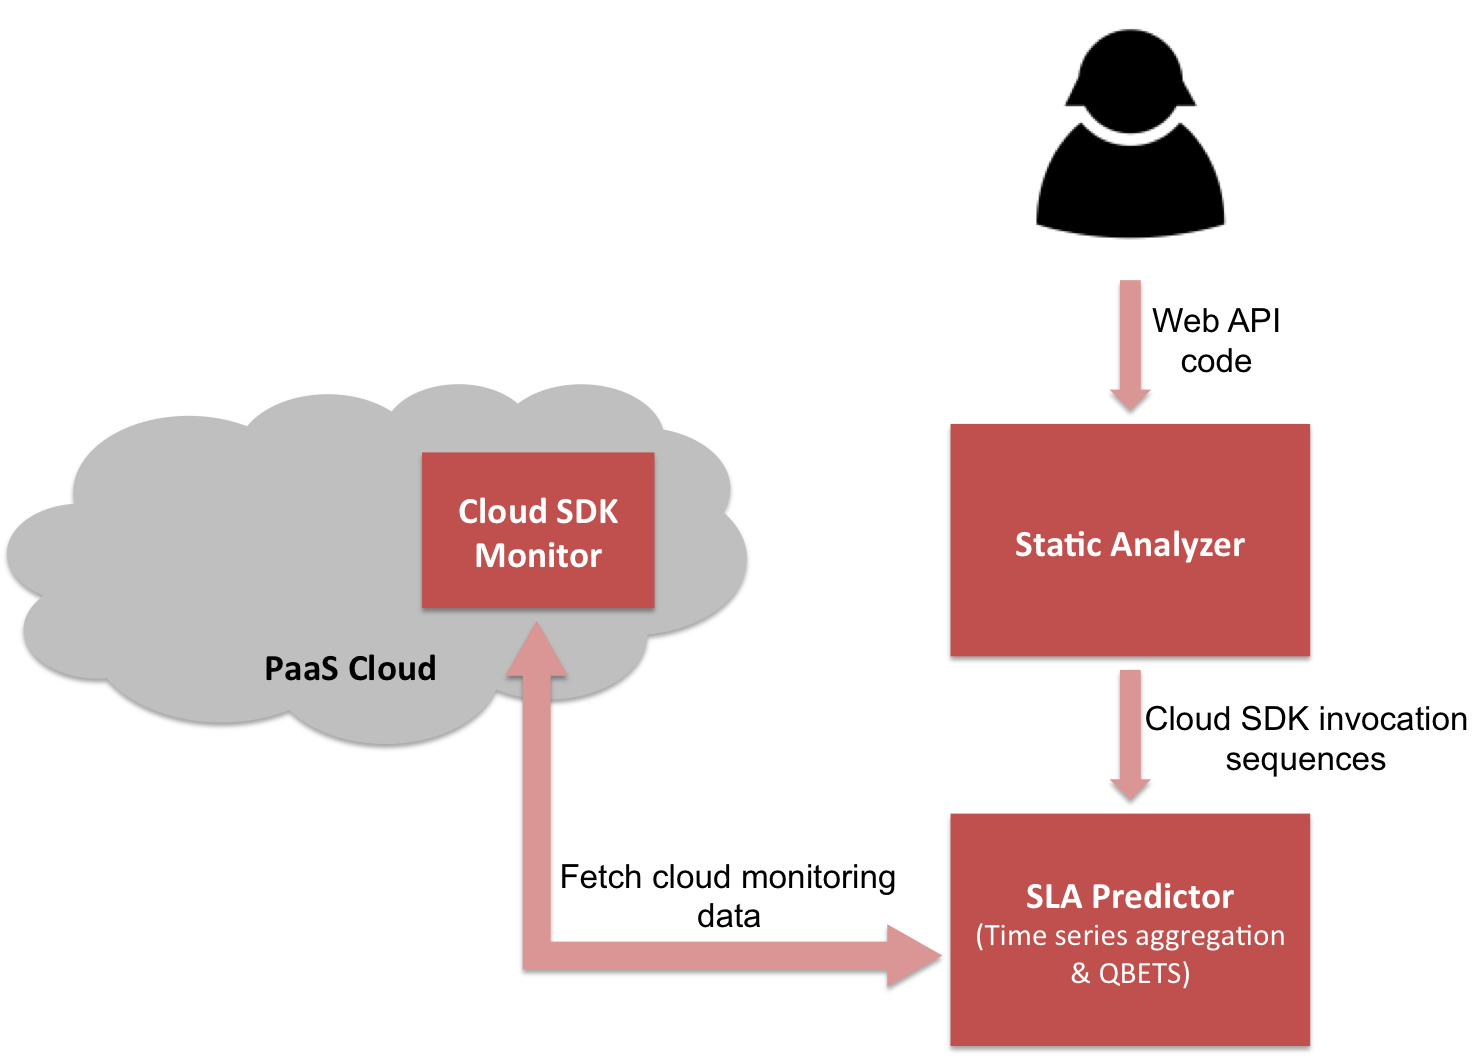
\includegraphics[scale=0.35]{cerebro_arch}
\caption{Cerebro architecture and component interactions.}
\label{fig:cerebro_arch}
\end{figure}

Figure~\ref{fig:cerebro_arch} illustrates how the Cerebro components interact with
each other during the prediction making process.  Cerebro can be
invoked when a web API is deployed to a PaaS cloud or at any time during the development
process to give developers insight into the worst case response time of their
applications.

Upon invoking Cerebro with a web API code, Cerebro
performs its static analysis on all operations in the API. For each
analyzed operation it produces a list of annotated cloud SDK invocation sequences --
one sequence per program path. Cerebro then prunes this list to eliminate duplicates.
Duplicates occur when a web API operation has
multiple program paths with the same sequence of cloud SDK invocations.
Next, for each pruned list Cerebro performs the following operations:
\begin{enumerate}
\item Retrieve (possibly compressed) benchmarking data from the monitoring agent 
for all SDK operations in each sequence. The agent returns
ordered time series data (one time series per cloud SDK operation).
\item Align retrieved time series across operations in time, and sum the aligned
values
to form a single \textit{joint} time series of the summed values for the 
sequence of cloud SDK operations.
\item Run QBETS on the aggregate time series with the 
desired $p$ and $c$ values to predict an upper bound. 
\end{enumerate}
Cerebro uses largest predicted value (across path sequences and operations) 
as its SLA prediction for the web API.
This process (SLA prediction) can be implemented
as a co-located service in the PaaS cloud or as a standalone utility.  We do 
the latter in our prototype.

As an example, suppose that the static analysis results in the
cloud SDK invocation sequence $<op_{1},op_{2},op_{3}>$ for
some operation in a web API. 
Assume that the monitoring agent has collected the following
time series for the three SDK operations:
\begin{itemize}
\item $op_{1}$: $[t_{0}: 5, t_{1}: 4, t_{2}: 6, ...., t_{n}: 5]$
\item $op_{2}$: $[t_{0}: 22, t_{1}: 20, t_{2}: 21, ...., t_{n}: 21]$
\item $op_{3}$: $[t_{0}: 7, t_{1}: 7, t_{2}: 8, ...., t_{n}: 7]$
\end{itemize}

Here $t_{m}$ is the time at which the $m^{th}$ measurement is taken.
Cerebro aligns the three time series according to timestamps, 
and sums the results
to obtain the following joint time series:
$[t_{0}: 34, t_{1}: 31, t_{2}: 35, ...., t_{n}: 33]$

If any operation is tagged as being inside a loop, where the loop
bounds have been estimated, Cerebro multiplies
the time series data corresponding to that 
operation by the loop bound estimate before aggregating. In cases where the operation 
is inside a data dependent loop, we request the time series data from 
the monitoring agent for its iterative datastore read benchmark 
for a number of entities that is equal to or larger than the annotation
and include it in the joint time series.

Cerebro passes the final joint
time series for each sequence of operations to QBETS, 
which returns the worst-case upper bound response time it predicts.
If the QBETS predicted value is $Q$ milliseconds, 
Cerebro forms the SLA as ``the web API will respond  in
under $Q$ milliseconds, $p$\% of the time''. 
When the web API has multiple operations, Cerebro estimates multiple 
SLAs for the API. 
If a single value is needed for the entire API regardless of operation,
Cerebro returns the largest 
predicted value as the final SLA (i.e. the worst case SLA for the API).

%Cerebro allows PaaS administrators to define API governance policies that 
%allow an application to be deployed only when its web APIs will meet a 
%pre-determined (or pre-negotiated) SLA target and to be notified 
%by the platform when such SLAs require renegotiation.


%this should go in the evaluation (where we discuss correctness), not here
%The QBETS implementation we use does not just generate one prediction when executed on
%some input time series. Rather, it generates a sequence of predictions -- one prediction per data point in the input
%time series. That is, it provides a trace of how the predictions change with each observed data point.
%When run on time series data gathered by our cloud SDK monitor,
%this would result in a prediction sequence with one entry per minute.
%We return the entire sequence of predictions generated by QBETS
%as the output. In situations where we just need a single prediction value, we pick the last prediction of the output
%sequence, and discard the rest.


%\section{Prototype Implementation}
%\label{sec:prototype_impl}
%We implemented a prototype of Cerebro that works with Google App Engine and AppScale cloud platforms.
The prototype analyzes web APIs implemented in Java, and makes SLA predictions for them.
%In this section we present the details of our prototype.

\subsection{Static Analyzer}
We implemented the static analyzer component of Cerebro using Soot~\cite{Vallee-Rai:2010:SJB:1925805.1925818}, a powerful
static analysis and code manipulation framework for Java. It supports performing a wide range of analyses on both Java source
code and byte code. Soot converts the input Java code into one of four intermediate representations (Baf, Jimple,
 Shimple and Grimp), and constructs the CFG for the code. It provides a number of common static
 analyses as built-in utilities, and also provides a set of programming APIs to enable developing custom
 analyses.
 
Our prototype static analyzer takes the compiled byte code of web applications as input. It uses the
Soot framework to transform byte code into Jimple, and from that it constructs the CFGs for 
all the Java methods in the exposed web API classes. Currently, our
prototype treats following classes as exposed web APIs:

\begin{itemize}
\item classes that extend the \textit{javax.servlet.HttpServlet} class (i.e. Java servlet implementations)
\item classes that bare the JAXRS \textit{@Path} annotation (i.e. JAXRS API implementations)
\item any other classes explicitly specified by the developer in a special configuration file
\end{itemize}
 
Our prototype then proceeds to analyze each of the public methods in the web API classes
using the algorithm described earlier. Each public method is considered a separate operation
in the web API, and hence given a separate execution time prediction.
All cloud SDK operations supported by Google App Engine
are grouped under the Java package name \textit{com.google.appengine.apis}. Whenever we detect
a function call node in a CFG, we check whether the call target belongs to the above package.
This way we can efficiently identify the cloud SDK invocations in the code.

We also use Soot's built-in loop extraction analysis
to detect loops in the code. In cases where loops contain cloud SDK calls, we attempt to estimate
the loop bounds using a loop bound prediction algorithm based on abstract interpretation~\cite{bygde2010static}. This
approach yields successful results with regard to data-independent loops. In case of data-dependent
loops (which is the more common case), we simply prompt the API developer to specify the loop iteration
count. We also support a non-interactive mode, where the developer can provide the maximum number of
records in the datastore (iterations) as a startup parameter to Cerebro.%, in which case the static analyzer will simply use the
%provided input value to annotate the cloud SDK calls in data-dependent loops.

\subsection{Watchtower}
We implemented Watchtower as a Java web application that can be deployed on Google App Engine and
AppScale. It is capable of benchmarking a wide range of cloud SDK operations
-- primarily the ones related to datastore and memcache. All benchmarking results are timestamped and 
saved in the datastore. Our implementation of Watchtower also benchmarks the iterative datastore read operation
with result set sizes 10, 100 and 1000. 

This implementation makes use of the job scheduling capabilities provided by Google App
Engine and AppScale. When deployed, it starts a cronjob in the cloud platform to invoke the benchmarking code
once every 60 seconds. Our implementation also exposes a set of REST APIs, which
are used by other components of Cerebro to retrieve the collected benchmarking data as time series.

\subsection{QBETS and SLA Predictor}
We use an implementation of QBETS written in C. We wrap this C program in a little bit of Go code, so some 
of its features are exposed as a web API. This web API is used by the static analyzer to pass in the extracted
cloud SDK invocation sequences, and other input parameters. We also have code for contacting Watchtower 
to retrieve the time series data required to make predictions, aggregating the time series, and then 
starting the QBETS analysis. 

\subsection{Using the Prototype}
To start using our prototype, one must first deploy the Watchtower application on the target cloud platform. 
Ideally Watchtower should be allowed to run for a several hours,
so that it can collect enough time series data for the QBETS analysis. Then,
an API developer who has implemented a web API for the cloud can build his/her code into a deployable
artifact (typically a .war file), and submit it to the static analyzer of Cerebro, along with the desired percentile
and upper confidence values (if not provided our prototype defaults to $p=95$ and $c=0.05$). This kicks off
the process for predicting SLAs for web API operations in the input web application.
%The static analyzer will extract
%the cloud SDK invocations from the web API code, and pass them along to the SLA predictor. The predictor
%will retrieve the time series data for cloud SDK operations from Watchtower, run QBETS and return the
%generated prediction values.

\vspace{-0.10in}
\section{Experimental Results}
\label{sec:results}
To empirically evaluate Cerebro, we conduct experiments using five open source, Google
App Engine applications.

\begin{description}
\item[StudentInfo] RESTful (JAX-RS) application for managing
students of a class (adding, removing, and listing student information).
\item[ServerHealth] Monitors, computes, and reports statistics for server
uptime for a given web URL.
\item[SocialMapper] A simple social networking application with APIs for
adding users and comments.
\item[StockTrader] A stock trading application that
provides APIs for adding users, registering companies, buying and selling
stocks among users. 
\item[Rooms] A hotel booking application with APIs
for registering hotels and querying available rooms.
\end{description}

These web APIs use the datastore
cloud SDK interface extensively. The Rooms web API also uses the
memcache interface. We focus on these two interfaces exclusively in this
study. We execute these applications in the Google App Engine public cloud 
(SDK v1.9.17)
and in an AppScale (v2.0) private cloud.  We instrument the programs to collect
execution time statistics for verification purposes only 
(the instrumentation data is not used to predict
the SLAs).  The AppScale private cloud used for testing was
hosted using four ``m3.2xlarge'' virtual machines running on a private
Eucalyptus~\cite{eucalyptus09} cloud.

%We instrument each of the five sample applications to measure the 
%time taken by their web APIs to execute the
%enclosed code. This is done by adding some extra Java code to each of the web APIs exposed by the sample applications.
%We ensure that the instrumentation does not alter the original web API code in anyway (i.e. the original algorithms, control flow
%and data flow are not impacted by the instrumentation). Then for each application we also
%implement a mechanism to output the measured execution times, so an external client can query and collect the execution
%times of the web APIs.

%We carry out each of our tests in two separate environments -- Google App Engine public cloud, and
%the AppScale private cloud. 
%The AppScale private cloud used for testing was powered by four m3.2xlarge virtual machines 
%running on a private Eucalyptus~\cite{eucalyptus09} cluster.

We first report the time required for Cerebro to perform its analysis and SLA prediction.
Across web APIs, Cerebro takes $10.00$ seconds on average, with a 
maximum time of $14.25$ seconds for StudentInfo.
These times include the time taken
by the static analyzer to analyze all the web API operations
and the time taken by QBETS to make predictions. For these results, the length of 
the time series collected by PaaS monitoring agent is $1528$ data points ($25.5$ hours of monitoring data). Since the QBETS analysis time depends on the length of the input time series, 
we also measured the time for 2 weeks of monitoring data ($19322$ data points) to provide
some insight into the overhead of SLA prediction.  Even in this case, Cerebro
requires only $574.05$ seconds ($9.6$ minutes).

\subsection{Correctness of Predictions}
\label{sec:correctness}

We first evaluate the correctness of Cerebro predictions.  A set of
predictions is \textit{correct} if the \textit{fraction} of measured 
response time values that fall below the Cerebro prediction is greater than 
or equal to the SLA target probability. 
For example, if the SLA probability is $0.95$ (i.e. $p=95$ in QBETS) for
a specific web API, then the Cerebro predictions are correct if at least
$95\%$ of the response times measured for the web API are smaller than their
corresponding Cerebro predictions. 

We benchmark each web API for a period of 15 to 20 hours.  During this time we
run a remote HTTP client that makes requests to the web APIs once every
minute.  The application instrumentation measures and records the response
time of the API operation for each request (i.e. within the application).
Concurrently and within the same PaaS system, we execute the Cerebro
PaaS monitoring agent which is an independently hosted application within the
cloud that benchmarks each SDK operation once every minute.

Cerebro predicts the web API execution times using only the cloud SDK
benchmarking data collected by Cerebro's PaaS monitoring agent. 
We configure Cerebro to predict an
upper bound for the $95^{th}$ percentile of the web API response time, with an
upper confidence of $0.01$. 

QBETS generates a prediction for \textit{every} value in the input time series 
(one per minute).  Cerebro reports the last one as the SLA prediction to the
user or PaaS administrator in production.  However, having per-minute predictions 
enables us to compare these predictions against actual web API execution
times measured during the same time period to evaluate Cerebro correctness. 
More specifically, we
associate with each measurement the prediction from the prediction time series
that most nearly precedes it in time.  The correctness fraction is computed
from a sample of $1000$ prediction-measurement pairs.

%align the sequence of predictions with the time series of actual
%execution time measurements, and check whether each prediction is equal to or
%higher than the corresponding measurement. We consider a sequence of 1000
%consecutive predictions and 1000 consecutive API execution time measurements,
%and compute the percentage of measurements that are less than or equal to the
%predicted values (a metric that we refer to as \textit{percentage accuracy}).

\begin{figure}
\centering
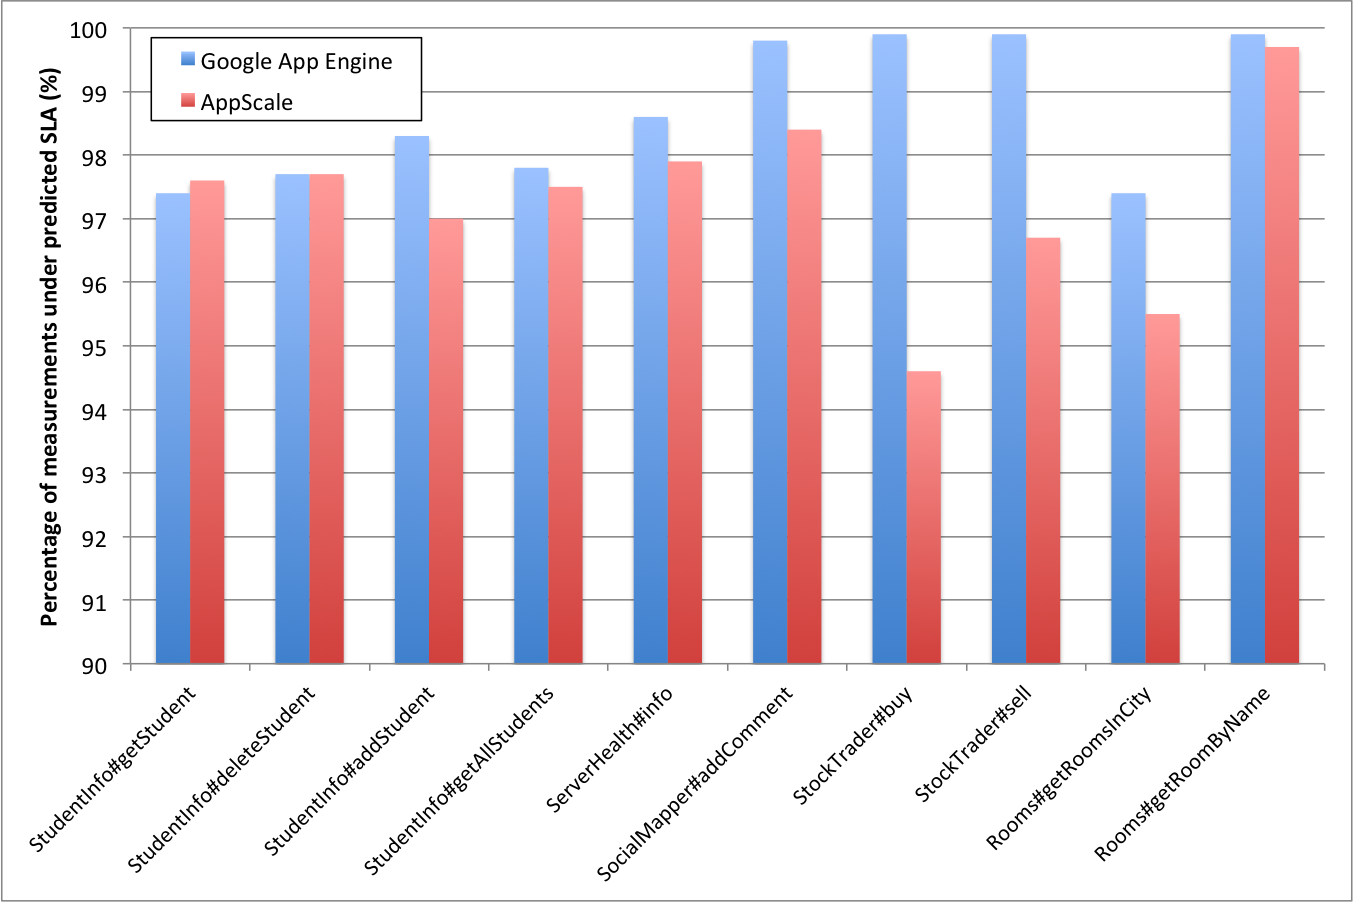
\includegraphics[scale=0.35]{accuracy_summary}
\caption{Cerebro correctness percentage in Google App Engine and AppScale cloud platforms.}
\label{fig:accuracy_summary}
\vspace{-0.2in}
\end{figure}

Figure~\ref{fig:accuracy_summary} shows the final results of this experiment.
Each of the columns in Figure~\ref{fig:accuracy_summary} corresponds 
to a single web API operation in 
one of the sample applications. The columns are labeled in the 
form of \textit{ApplicationName\#OperationName}, a convention 
we will continue to use in the rest of the paper. %To maintain clarity in the figures we do not 
%illustrate the results for all web API operations in the sample applications. Instead we present the results for a selected set of 
%web API operations covering all five sample applications. We note that other web API operations we tested also produce
%very similar results.

Since we are using Cerebro to predict the $95^{th}$ percentile of the API
response times, Cerebro's predictions are correct when at 
least $95\%$ of the measured response times are
less than their corresponding predicted upper bounds. According to
Figure~\ref{fig:accuracy_summary}, Cerebro achieves this goal for all the
applications in both cloud environments. 
%The lowest percentage accuracy observed in our tests is 94.6\% (in the case
%of StockTrader\#buy on AppScale), which is also very close to the target of
%95\%.  Such minor lapses below 95\% are acceptable anyway, since we expect
%percentage accuracy value to be gently fluctuating around some average value
%over time (a phenomenon that will be explained in our later results).
%Overall, this result shows us that Cerebro produces highly accurate SLA
%predictions for a variety of applications running on two very different cloud
%platforms.

The web API operations illustrated in Figure~\ref{fig:accuracy_summary} cover
a wide spectrum of scenarios that may be encountered in real world.
StudentInfo\#getStudent and StudentInfo\#addStudent are by far the simplest
operations in the mix. They invoke a single cloud SDK operation each, and
perform a simple datastore read and a simple datastore write respectively. As
per our survey results, these alone cover a significant portion of the web
APIs developed for the App Engine and AppScale cloud platforms (1 path through
the code, and 1 cloud SDK call).  The StudentInfo\#deleteStudent operation
makes two cloud SDK operations in sequence, whereas
StudentInfo\#getAllStudents performs an iterative datastore read.  In our
experiment with StudentInfo\#getAllStudents, we had the datastore preloaded
with $1000$ student records, and Cerebro was configured to use a maximum entity
count of $1000$ when making predictions.

ServerHealth\#info invokes the same cloud SDK operation three times in
sequence. Both StockTrader\#buy and StockTrader\#sell have multiple paths
through the application 
(due to branching), thus causing Cerebro to make multiple
sequences of predictions -- one sequence per path. The results shown in
Figure~\ref{fig:accuracy_summary} are for the longest paths which consist of
seven cloud SDK invocations each. According to our survey, $99.8\%$ of the
execution paths found in Google App Engine applications have seven or 
fewer cloud SDK
calls in them. Therefore we believe that the StockTrader web API
represents an important upper bound case. 

Rooms\#getRoomByName
invokes two different cloud SDK interfaces, namely datastore and memcache.
Rooms\#get\-AllRooms is another operation that consists of an iterative
datastore read. In this case, we had the datastore preloaded with $10$ entities,
and Cerebro was configured to use a maximum entity count of $10$. 
%It is indeed encouraging to see how Cerebro manages to produce highly accurate predictions
%for such a wide range 
%of web API implementations and runtime scenarios on two cloud platforms.

\subsection{Tightness of Predictions}

In this section we discuss the tightness of the predictions generated by Cerebro. 
Tightness is a measure of how closely the predictions
bound the actual response times of the web APIs. 
Note that it is possible to perfectly achieve the correctness goal
by simply predicting overly large values for web API response times. For example, if Cerebro were to
predict a response time of several years for exactly $95\%$ of the web API
invocations and zero for the others, it would likely
achieve a correctness percentage of $95\%$.  From a practical perspective,
however, such an extreme upper bound is not useful as the basis for an SLA. 
%This parameter is just as important as the percentage of measurements that fall under the predicted SLA values. 
%Note that Cerebro can achieve a very high percentage accuracy level by simply generating a 
%sequence of large predictions. But such results will obviously be of very little use to the API
%developers. For the predictions to be useful and meaningful, they should be very close to the actual response times of the web APIs.

\begin{figure}
\centering
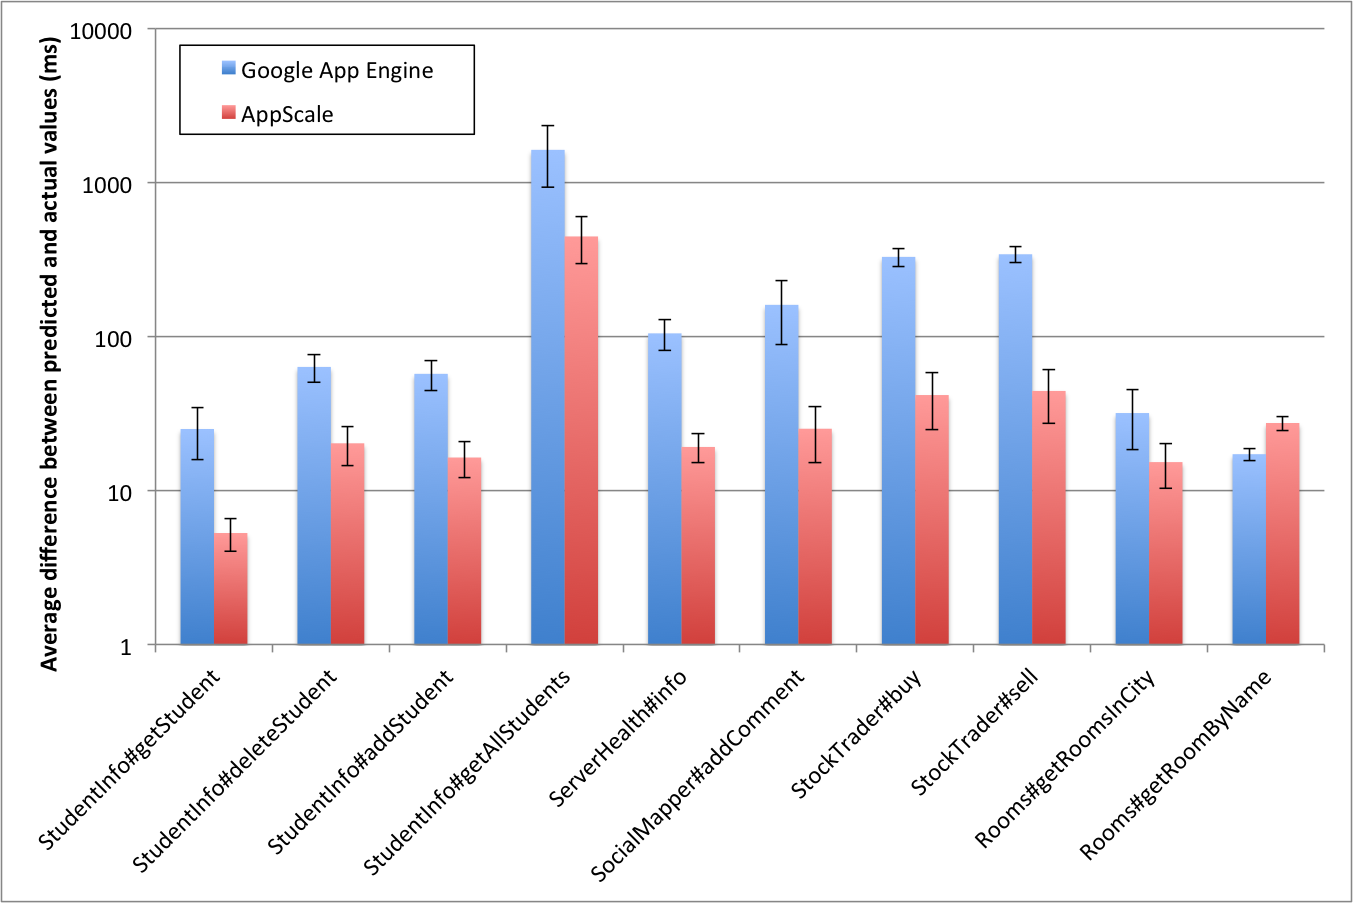
\includegraphics[scale=0.35]{diff_summary}
\caption{Average difference between predictions and actual response times in
Google App Engine and AppScale. The y-axis is in log scale.}
\label{fig:diff_summary}
\vspace{-0.2in}
\end{figure}

Figure~\ref{fig:diff_summary} depicts the average difference between predicted
response time bounds and actual response times for
our sample web APIs when running in the App Engine and AppScale clouds. 
These results were obtained considering a sequence of $1000$ 
consecutive predictions (of $95^{th}$ percentile) and the averages are
computed only for correct predictions (i.e. ones above their corresponding
measurements).
%Within these prediction sequences only the cases 
%where the predicted value was larger than the corresponding actual execution time was taken into account. Based on the results
%presented earlier, we know that this case occurs at least 95\% of the time.

According to Figure~\ref{fig:diff_summary}, Cerebro generates fairly tight 
SLA predictions for most web API operations considered in the experiments. In fact,
$14$ out of the $20$ cases illustrated in the figure show average difference
values less than $65$ms. In a few cases, however, the bounds differ from the
average measurement substantially:
\begin{itemize}
\vspace{-0.05in}
\item StudentInfo\#getAllStudents on both cloud platforms
\vspace{-0.05in}
\item ServerHealth\#info, SocialMapper\#addComment, StockTrader\#buy and StockTrader\#sell on App Engine
\vspace{-0.05in}
\end{itemize}

%To understand why Cerebro generates conservative predictions for some operations we further 
%investigate the performance characteristics of them. We take StudentInfo\#getAllStudents
%operation on App Engine as a case study, and analyze its execution time measurements in depth. 
%This is the case which exhibits the largest average difference between predicted and actual execution times.

\begin{figure}
\centering
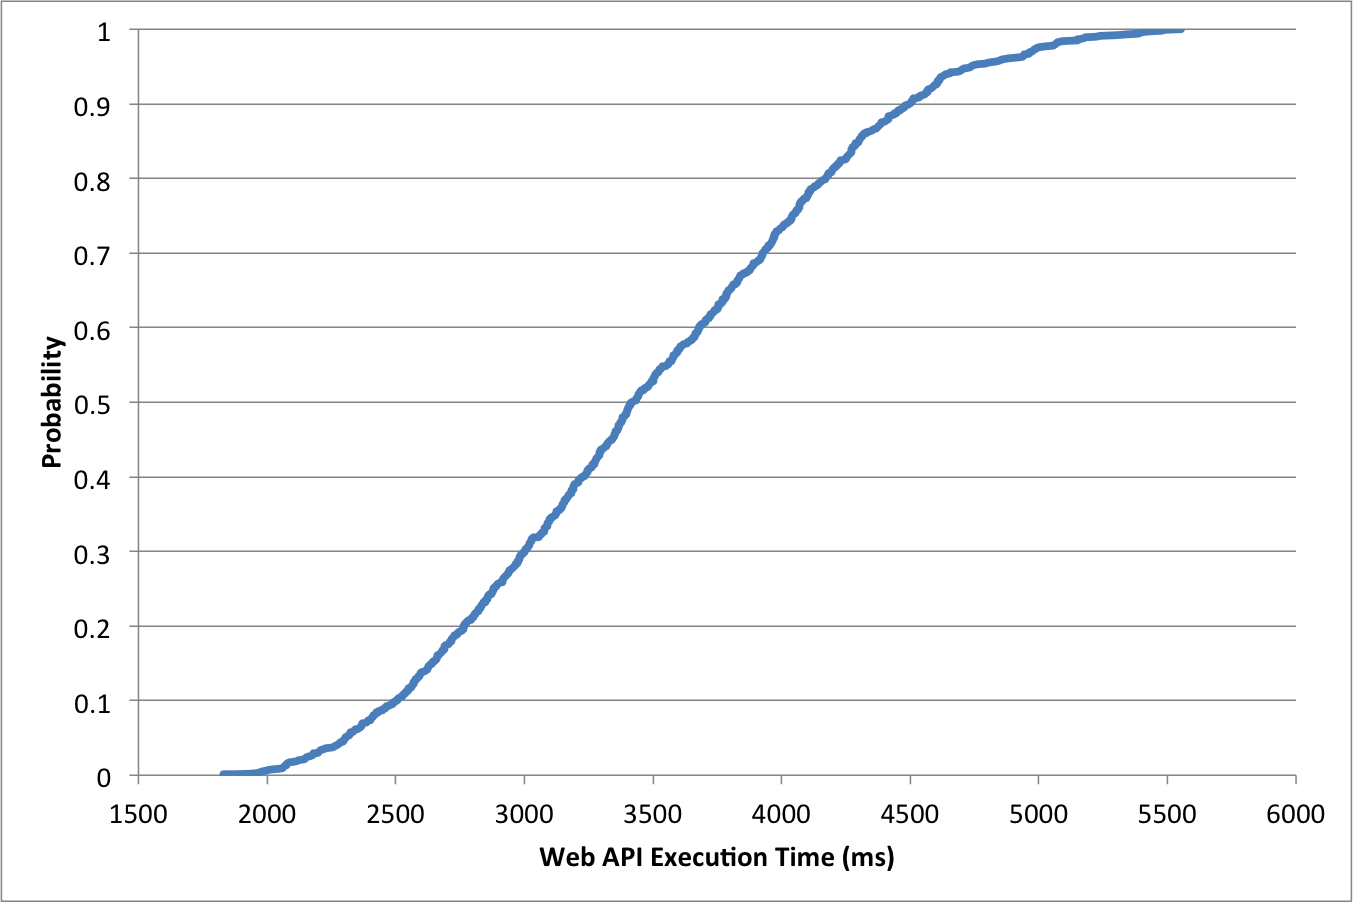
\includegraphics[scale=0.35]{get_all_students_cdf}
\caption{CDF of measured executions times of the StudentInfo\#getAllStudents operation on App Engine.}
\label{fig:get_all_students_cdf}
\vspace{-0.2in}
\end{figure}

Figure~\ref{fig:get_all_students_cdf} shows the empirical cumulative
distribution function (CDF) of measured execution times for the 
StudentInfo\#getAllStudents on
Google App Engine (one of the extreme cases). 
This distribution was obtained by considering the application's instrumentation 
results gathered within a window of $1000$ minutes. 
The average of this sample is $3431.79$ms, and the $95^{th}$ percentile
from the CDF is $4739$ms.  Thus, taken as a distribution, the ``spread''
between the average and the $95^{th}$ percentile is more
than $1300$ms.  

% ----- Hiranya: The following observation is wrong. Cerebro spread is 1600ms, not 1100ms -----

%For this case (column 4 in Figure~\ref{fig:diff_summary}), Cerebro's
%spread is approximately $1100$ms.  Thus Cerebro appears to be generating an
%accurate estimate of the $95^{th}$ percentile for this data.  That is, a
%response time SLA of $1100$ms would likely be achievable with probability
%at least $0.95$ 
%for the StudentInfo\#getAllStudents web API when the application is
%running in Google App Engine. 

From this, it becomes evident that StudentInfo\#getAll\-Students 
records very high execution times frequently. 
In order to incorporate such high outliers, Cerebro must be conservative 
and predict large values for
the $95^{th}$ percentile. This is a required feature to ensure that 95\% or more 
API invocations have
execution times under the predicted SLA. But as a consequence, the average 
distance between the 
measurements and the predictions increases significantly.

We omit a similar analysis of the other cases in the interest of brevity 
but summarize the tightness results as indicating that Cerebro achieves a
bound that is ``tight'' with respect to the percentiles observed by sampling
the series for long periods. 
%Our analyses with other operations for which
%Cerebro generates conservative bounds have also shown similar results. That is, when the performance of the web API is highly variable and
%when its execution time distribution contains
%many high outliers, Cerebro produces predictions that are less tight. In other words, 
%Cerebro trades off tightness of the predictions for their accuracy.

%\begin{figure}
%\centering
%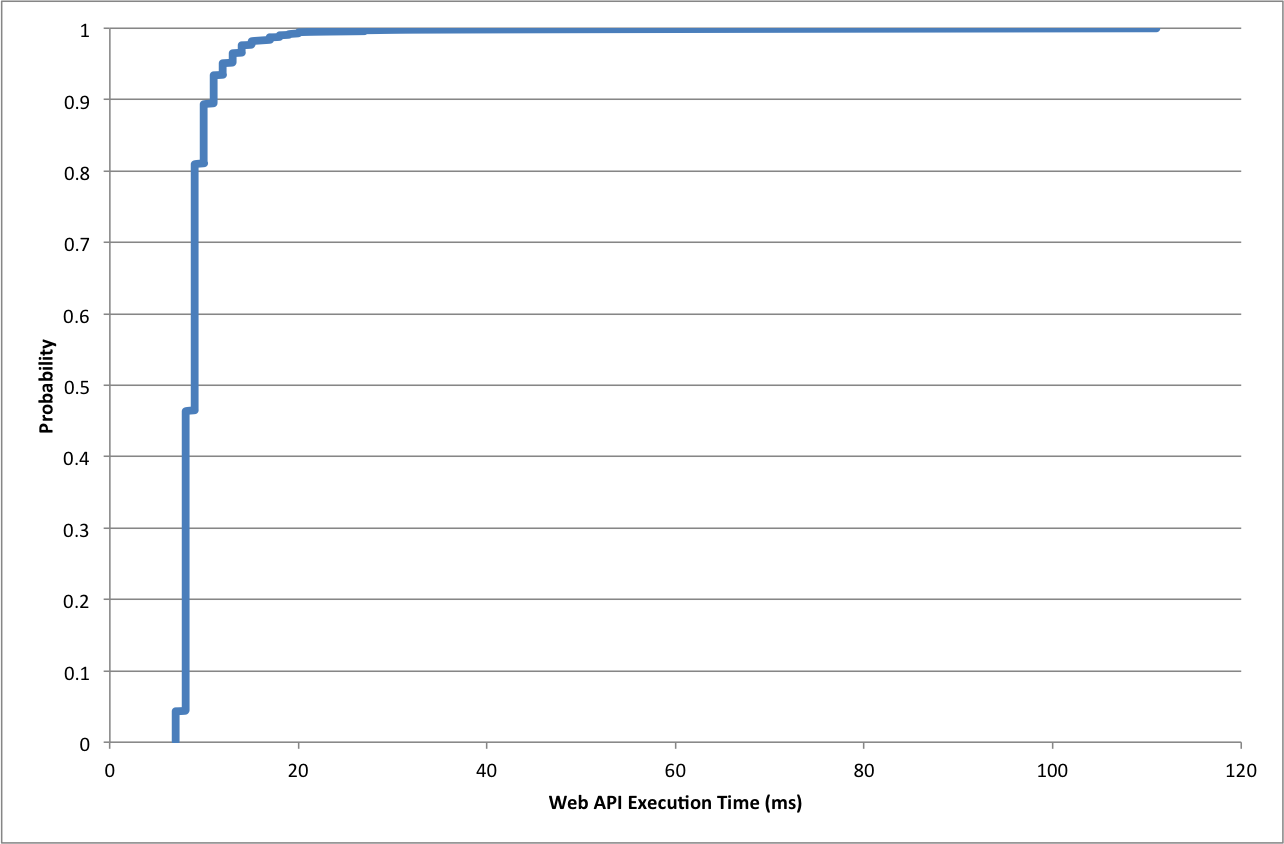
\includegraphics[scale=0.35]{get_student_cdf}
%\caption{CDF of measured response times of the StudentInfo\#getStudent operation on AppScale.}
%\label{fig:get_student_cdf}
%\end{figure}
%
%We also investigate one of the web API operations that result in very tight predictions. 
%Figure~\ref{fig:get_student_cdf} shows the CDF of the measured execution times for the StudentInfo\#getStudent operation on
%AppScale. Again we are considering a sample time frame of 
%$1000$ minutes in the graph.
%This particular distribution has a average of $9.19$ms and a $95^{th}$
%percentile of $12$ms. 
%Given that only 19\% of the values are larger than the mean, 
%and only 2\% of the values are larger than 18ms (twice the mean), 
%we see that this distribution is much more stable and have very few high outliers. This enables Cerebro to generate much
%tighter predictions, without compromising the accuracy of the results. Based on these outcomes we can conclude that Cerebro produces
%very tight upper bound predictions for web APIs whose performance is more stable over time. %For APIs with highly variable performance
%traits resulting in many high outliers, Cerebro generates more conservative and less tight predictions.
%At this point it is worth reaffirming that Cerebro does not consider the actual execution time measurements of the web APIs when
%making SLA predictions for them. It only has access to the cloud SDK benchmarking data gathered by Watchtower. 
%We consider Cerebro's ability to understand the variability of a web API's performance by only looking at the cloud SDK
%benchmarking data, as one of its strengths.

Another interesting observation we can make regarding the tightness of
predictions is that the predictions made in the AppScale cloud platform are
significantly tighter than the ones made in Google App Engine
(Figure~\ref{fig:diff_summary}). 
%Five out of the six scenarios in which Cerebro has generated conservative
%predictions are from App Engine.  Furthermore,
For nine out of the ten operations tested, Cerebro has generated tighter
predictions in the AppScale environment. This is because web API performance
on AppScale is far more stable and predictable thus resulting in fewer
measurements that occur far from the average.

The reason why AppScale's performance is more stable over time is because it is
deployed on a set of closely controlled 
and monitored cluster of virtual machines (VMs) that use a private
Infrastructure-as-a-Service (IaaS) cloud to implement isolation.  In particular, the 
VMs assigned to AppScale do not share nodes with ``noisy neighbors'' in our
test environment.  In contrast, Google App Engine does not expose the
performance characteristics of its multi-tenancy.  While it operates at vastly
greater scale, our test applications also exhibit wider variance of web API
response time when using it.
%We have total control
%over how much resources are assigned to the VMs, and we ensure that they run in total isolation from the other processes 
%running on the underlying hardware.
%This is not the case when running our sample applications on App Engine, where we have no control over 
%the underlying VMs, hardware and the
%scheduling mechanism. Another related, but interesting outcome of these results is that large-scale public cloud platforms like App Engine, while
%highly scalable, may not be able to support tight performance SLAs. Their performance is subject to high variations making it difficult to always support attractive
%performance guarantees. Small private cloud platforms on the other hand can provide much better, consistent and stable performance guarantees, albeit their
%poor scalability. %From an organization's point of view this could be a strong motivator to adopt private cloud over public clouds.
Cerebro, however, is able to predict a correct and tight SLAs for applications
running in either platform: the lower variance private
AppScale PaaS, and the extreme scale but more varying Google App Engine PaaS.

\subsection{Duration of Prediction Validity}

%So far we have examined the accuracy and tightness of the predictions produced by Cerebro. In this section we 
%focus on the validity period of the Cerebro predictions.
%
%Cloud platforms are highly dynamic environments. Some of the changes that may occur in such an environment include:
%\begin{itemize}
%\item addition or removal of hardware resources/VMs/containers,
%\item software updates and upgrades, and
%\item component failures.
%\end{itemize}

%When the platform is subject to such significant and frequent changes, performance SLAs predicted for the web APIs deployed on that
%platform may not hold correct forever. Given enough time the APIs may start violating the predicted SLAs consistently. Therefore, for any
%given SLA prediction we need to have an approximate idea of how long that prediction is going to be valid for. In others words, we need
%to know how long it would take before a predicted SLA value cannot be considered correct. We refer to this time period as the 
%\textit{validity period} of a prediction.

%Ideally we want the validity period of a Cerebro prediction to be infinity. That is, once an SLA prediction has been made for a web API it
%should remain correct forever. If that was the case, the API performance would never degrade to a level where it
%consistently exceeds the originally predicted execution time upper bound. But due to the dynamic nature of the cloud platforms such
%behavior is highly unlikely. From a practical standpoint we can expect the prediction validity period to be some finite duration. 

%We believe
%it is important that cloud administrators be informed about the validity period of predictions so that they can periodically reassess the web
%API SLAs. For example they can run Cerebro periodically (before the prediction validity period expires) on the deployed web APIs to check
%if the predicted execution times have degraded to such a level where they no longer meet the organizational standards for API
%response times. 

To be of practical value to PaaS administration, the duration over which a
Cerebro prediction remains valid must be long enough to allow appropriate
remedial action when load conditions change, and the SLA is in danger of being
violated.  In particular, SLAs must remain correct for at least the time
necessary to allow human responses to changing conditions such as
the commitment of more resources to web APIs that are in violation or alerts
to support staff that customers may be calling to claim SLA breach.  Ideally,
each prediction should persist as correct for several hours or more to match
staff response time to potential SLA violations.

%If that is the case, the cloud administrators can take some remedial actions like 
%committing more resources to the deployed APIs,
%replicating them (horizontal scaling), or notifying the respective API developers about the impending performance issues. However,
%for this to be practical, the validity period of Cerebro predictions should at least be several hours. If the validity period is in the order of minutes,
%a lot of computing time and manpower will be wasted recomputing Cerebro predictions and evaluating the results. Also, given that
%modern cloud platforms are used to host thousands of web APIs, such aggressive re-computation of predictions may not be scalable.

However, determining when a Cerebro-predicted SLA becomes invalid is
potentially complex. For example, given the definition of correctness
described in Subsection~\ref{sec:correctness}, it is possible to report an SLA violation
when the running tabulation of correctness percentage falls below the target
probability (when expressed as a percentage).  However, if this metric is
used, and Cerebro is correct for many consecutive measurements, a sudden
change in conditions that causes the response time to persist at a higher
level will not immediately trigger a violation.  For example, Cerebro might be
correct for several consecutive months and then incorrect for several
consecutive weeks before the overall correctness percentage drops below $95\%$
and a violation is detected.  If the SLA is measured over a year, such time
scales may be acceptable but we believe that PaaS administrators would
consider such a long period of time where the SLAs were continuously in
violation unacceptable.
Thus we propose a more conservative approach to measuring the duration over
which a prediction remains valid than simply measuring the time until the
correctness percentage drops below the SLA-specified value.
%Before we can analyze the validity period of Cerebro predictions, we need to
%develop a model for detecting when a predicted SLA has become invalid. 

Suppose at time $t$ Cerebro predicts value $Q$ as the $p$-th percentile of
some API's execution time.  If $Q$ is a correct and tight prediction,
the probability of API's next measured response time being greater than 
$Q$ is $1-(0.01p)$.  If the time series consists of independent
measurements then the probability of seeing $n$ consecutive values greater
than $Q$ (due to random chance) is $(1-0.01p)^n$. 
For example, using the $95^{th}$ percentile, the probability of seeing $3$
values in a row larger than the actual percentile (purely due to random chance)
is $(0.05)^3 = 0.00012$ or about $1$ in $8333$.

This calculation is conservative with respect to autocorrelation. That is, if
the time series is stationary but autocorrelated, then the number of consecutive 
values above the $95^{th}$ percentile that correspond to a probability of
$0.0012$ is larger than $3$.  For example, in previous
work~\cite{Nurmi:2007:QQB:1791551.1791556}
using an artificially generated AR(1) series, 
we observed that $5$ consecutive values above the $95^{th}$ percentile
occurred with probability $0.00012$ when the first autocorrelation was $0.5$,
and $14$ when the first autocorrelation was $0.85$.  Thus using an independence
assumption for the series to determine the number of consecutive values above
$Q$ that constitute a ``rare event'' (indicating a possible change in
conditions) is conservative.

In particular, for the $95^{th}$ percentile, we measure the time from when
Cerebro makes a bounds prediction until we observe $n=3$ consecutive
measurement values above that prediction as being the time duration over which
the prediction is valid. We refer to this duration as the \textit{validity duration}.  
Tables~\ref{tab:gae_validity} and~\ref{tab:as_validity} present these durations
for Cerebro predictions in Google App Engine and AppScale
respectively.

%\begin{table}[tdp]
\begin{table}
\caption{Prediction validity period distributions of different operations in
App Engine. Validity durations were computed by observing $3$ consecutive SLA
violations. $5^{th}$ and $95^{th}$ columns represent the 5th and 95th 
percentiles of the
distributions respectively. All values are in hours.
\label{tab:gae_validity}
}
\begin{center}
\begin{tabular}{|c|p{1cm}|p{1cm}|p{1cm}|}
\hline
Operation & $5^{th}$ & Average & $95^{th}$ \\ \hline
StudentInfo\#getStudent & 7.15 & 70.72 & 134.43 \\ \hline
StudentInfo\#deleteStudent & 2.55 & 37.97 & 94.37 \\ \hline
StudentInfo\#addStudent & 1.45 & 26.8 & 64.78 \\ \hline
ServerHealth\#info & 1.41 & 39.22 & 117.71 \\ \hline
Rooms\#getRoomByName & 7.24 & 70.47 & 133.36 \\ \hline
Rooms\#getRoomsInCity & 2.08 & 30.12 & 82.58 \\ \hline
\end{tabular}
\end{center}
\vspace{-0.1in}
\end{table}

\begin{table}
\caption{Prediction validity period distributions of different operations in
AppScale. Validity periods were computed by observing $3$ consecutive SLA
violations. $5^{th}$ and $95^{th}$ 
columns represent the 5th and 95th percentiles of the
distributions respectively. All values are in hours.
\label{tab:as_validity}
}
\begin{center}
\begin{tabular}{|c|p{1cm}|p{1cm}|p{1cm}|}
\hline
Operation & $5^{th}$ & Average & $95^{th}$ \\ \hline
StudentInfo\#getStudent & 6.1 & 60.67 & 115.24 \\ \hline
StudentInfo\#deleteStudent & 6.08 & 60.21 & 114.32 \\ \hline
StudentInfo\#addStudent & 6.1 & 60.67 & 115.24 \\ \hline
ServerHealth\#info & 6.29 & 54.53 & 108.14 \\ \hline
Rooms\#getRoomByName & 6.07 & 59.18 & 112.28 \\ \hline
Rooms\#getRoomsInCity & 1.95 & 33.77 & 84.63 \\ \hline
\end{tabular}
\end{center}
\vspace{-0.2in}
\end{table}

%Next we shall assume that individual SLA
%violations are independent events; i.e. one SLA violation does not depend on
%another SLA violation.  Then, the probability of API violating the predicted
%SLA $n$ times in a row is $(1-0.01p)^n$, if $Q$ is a valid prediction.
%Therefore, if we state that the predicted SLA is invalid after observing $n$
%consecutive violations, the probability of us being correct would be $1 -
%(1-0.01p)^n$. 
%Notice that this value increases with $n$. 

%This implies that we can use consecutive SLA violations made by the API as an indicator of the SLA becoming
%invalid. Larger the number of consecutive violations we observe, more confident we can be about considering the SLA as invalid. 
%Hence for some $n$, if we observe
%the $n$-th consecutive violation at time $t^\prime$, we can consider the duration $t^\prime - t$ as the validity period of the prediction made 
%at time $t$. By the previous argument, the probability of this being an accurate approximation of validity period is $1 - (1-0.01p)^n$.

%Lets consider an example to further clarify this notion. Assume that for some web API at time $t$ Cerebro produces value $Q$ as the 
%prediction of the 95th percentile. Therefore after time $t$, the probability of the API violating this predicted SLA is 0.05, provided
%that $Q$ is a correct prediction. Similarly, if $Q$ is an accurate SLA prediction, and SLA violations are independent events, the probability of the API
%violating the SLA 3 times in a row would be $0.05^3$ or 0.000125. Hence after observing 3 consecutive violations the probability of $Q$
%being an incorrect prediction is $(1 - 0.000125)$ or 0.999875. If we want to be even more confident about detecting invalid SLAs, 
%we can look for an even higher
%number of consecutive SLA violations (i.e. higher $n$).  
%Based on the value they choose for $n$ the validity period of the predictions can be determined
%with a specific level of certainty.

%To evaluate the validity period of Cerebro predictions, we benchmark some of our sample applications for a period of 5 to 6 days on both
%App Engine and AppScale. We also run Watchtower on the same cloud platforms during this period. Then we run Cerebro using
%the Watchtower data to make per-minute SLA predictions (95th percentile; i.e $p=95$) for the entire duration of the tests. Next we choose a sequence of predictions
%in 15 minute intervals. For each of the selected predictions we try to find the time until 3 consecutive violations (i.e $n=3$) by scanning ahead into the trace of
%actual execution times gathered by directly benchmarking the web APIs. This provides us with a distribution of prediction validity periods where
%each validity period has a certainty level of 0.999875.
%However, for some predictions we are not able to find 3 consecutive violations in the traces of actual API execution times. We include
%such cases in the distribution by right censoring. That is, we consider the end of trace as the time to 3 consecutive violations for such cases.

%\begin{figure}
%\centering
%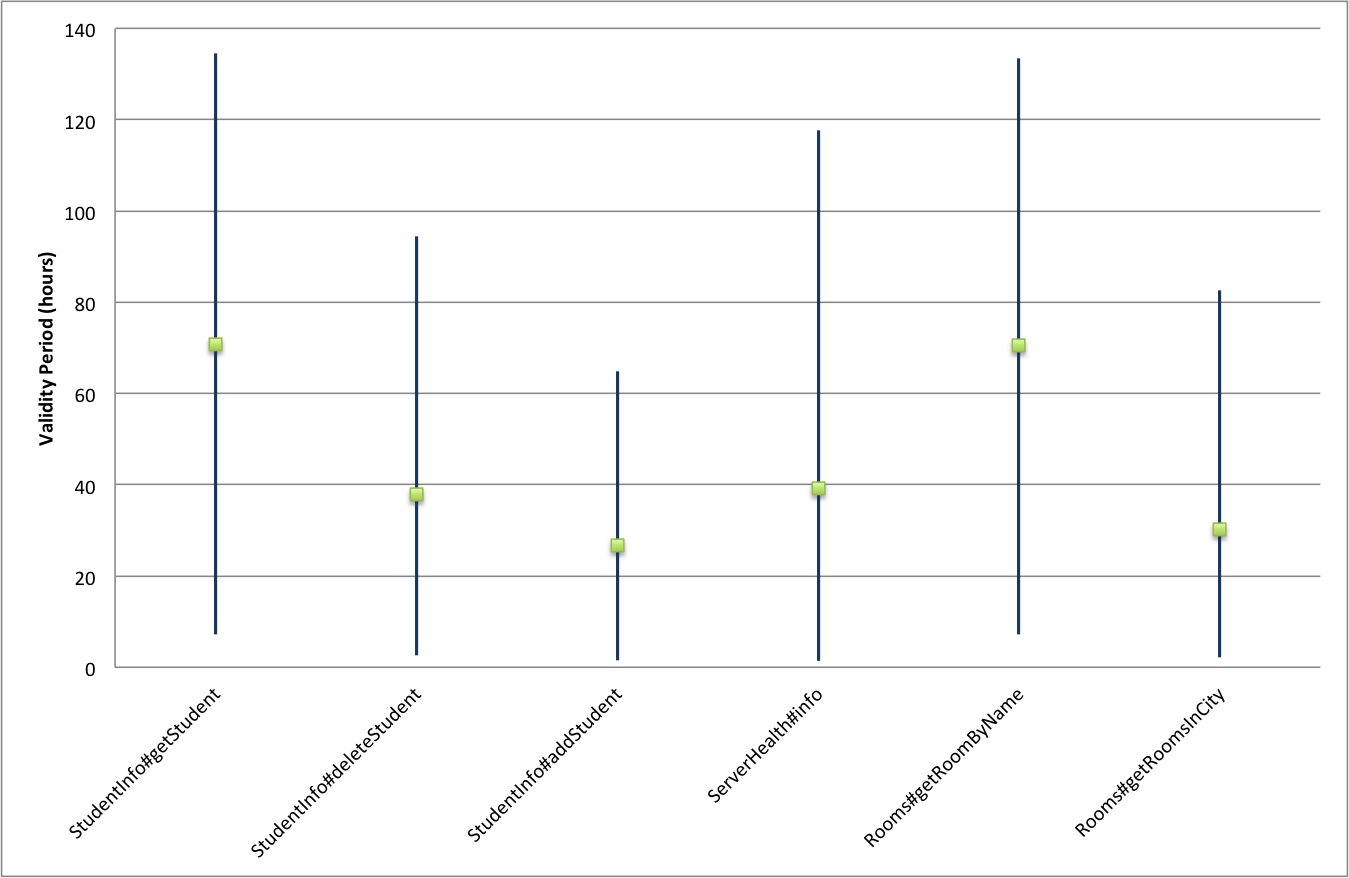
\includegraphics[scale=0.35]{gae_validity}
%\caption{Prediction validity period distributions of different operations in App Engine. The vertical lines indicate the range between the 5th and 95th percentiles of the distributions. The green markers represent the means. Validity periods were computed by observing 3 consecutive SLA
%violations.}
%\label{fig:gae_validity}
%\end{figure}


%\begin{figure}
%\centering
%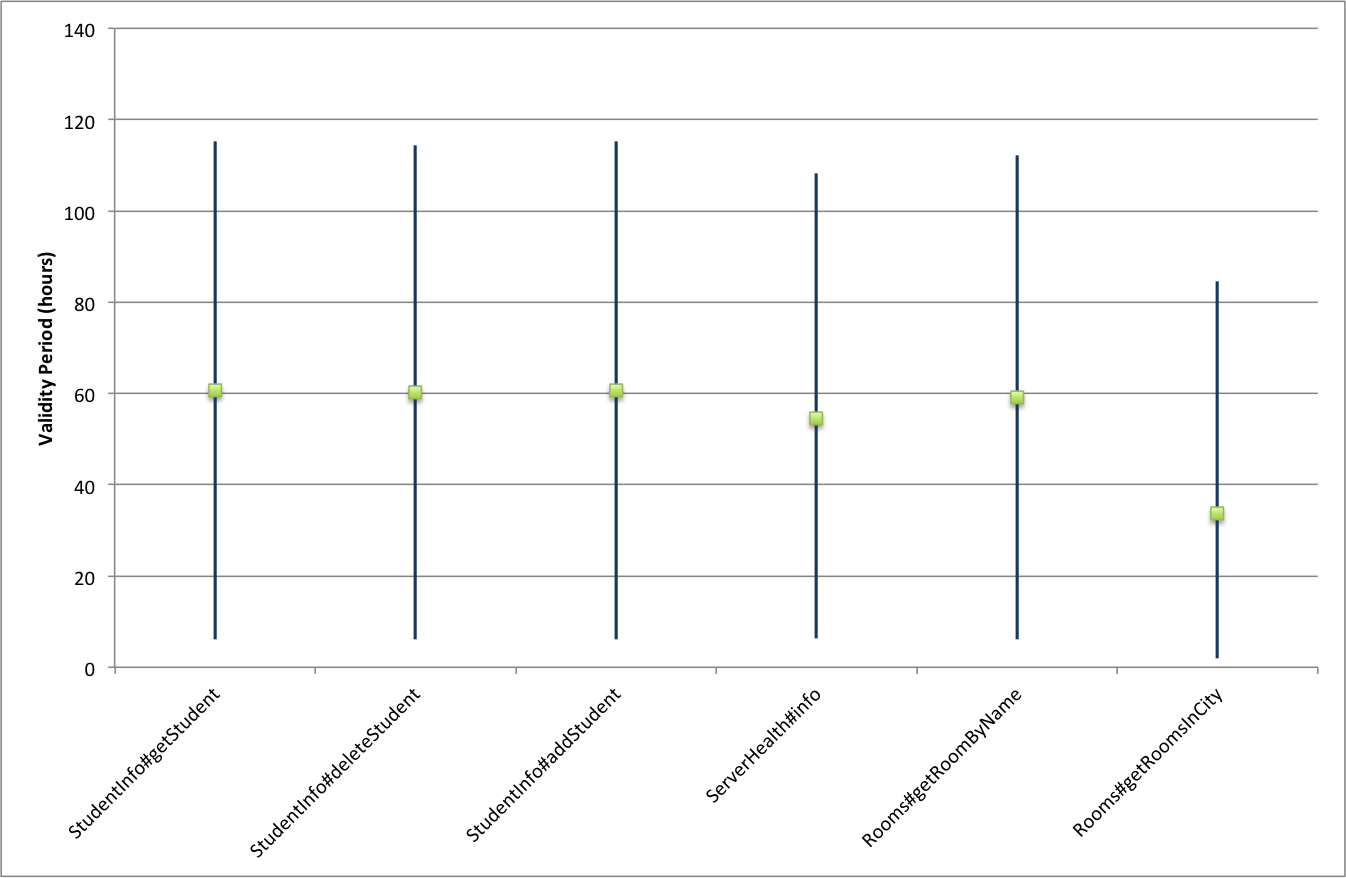
\includegraphics[scale=0.35]{as_validity}
%\caption{Prediction validity period distributions of different operations in AppScale. The vertical lines indicate the range between the 5th and 95th percentiles of the distributions. The green markers represent the means. Validity periods were computed by observing 3 consecutive SLA violations.}
%\label{fig:as_validity}
%\end{figure}

%Table~\ref{tab:gae_validity} shows a summary of the validity period distributions in App Engine. 
%The
%vertical lines represent the range from 5th to 95th percentiles. The square shaped markers on the lines indicate the means of the respective distributions.  
From Table~\ref{tab:gae_validity} 
the average validity duration for all 6 operations considered in App Engine is
longer than $24$ hours. The lowest average value observed is $26.8$ hours, 
and that is for the StudentInfo\#addStudent operation. If we
just consider the $5^{th}$ percentiles of the distributions, they are 
also longer than $1$ hour. The smallest $5^{th}$ percentile value of 
$1.41$ hours is 
given by the ServerHealth\#info operation. This result implies that if we use 
$3$ consecutive violations as a cue for detecting invalid SLAs,
Cerebro predictions made on Google App Engine would be valid for at least
$1.41$ hours or more, at least 95\% of the time.

By comparing the distributions for different operations we can conclude that
API operations that perform a single basic datastore or memcache read tend to
have longer validity durations. In other words, those cloud SDK operations have
fairly stable performance characteristics in Google App Engine. 
This is reflected in
the $5^{th}$ percentiles of StudentInfo\#getStudent and Rooms\#getRoomByName. 
Alternatively
operations that execute writes, iterative reads or long sequences of cloud SDK
operations have shorter prediction validity durations.

For AppScale, 
the smallest average validity period of $33.77$ hours is observed from the
Rooms\#getRoomsInCity operation. All other operations tested in 
AppScale have average prediction validity periods greater
than $54$ hours. The lowest $5^{th}$ percentile value in the 
distributions, which is 1.95 hours, is 
also shown by Rooms\#getRoomsInCity. This means, the SLAs predicted for
AppScale would hold correct for at least $1.95$ hours or more, 
at least 95\% of the time.
%Other operations have 5th percentile values greater than 6 hours. 
The relatively smaller validity period values computed for the
Rooms\#getRoomsInCity operation indicates that the performance of 
iterative datastore reads is subject to some variability 
in AppScale.

%Comparatively, the validity duration recorded in the AppScale
%cloud platform are longer than the ones seen in Google App Engine. 
%
%This is because compared to App Engine our
%test AppScale private cloud is much less dynamic. App Engine is a very large PaaS cloud that is served by thousands of
%nodes possibly distributed over multiple data centers. It is comprised of many components that are not under our control,
%and the entire cloud platform is used by thousands of users worldwide to deploy applications. Such a large scale and
%shared system has to endure a myriad of changes in any given moment (e.g. autoscaling of hardware resources, 
%changing application load, component failures etc.). This behavior affects the performance of the cloud SDK operations, which
%in turns affects the performance SLAs of high-level user code. In contrast, our AppScale
%private cloud is small, deployed on a handful of nodes that are under our control, and during our testing phase it was dedicated
%to running Watchtower and other sample applications. Therefore it is a much more stable environment compared to 
%App Engine -- a fact that is reflected in the calculated prediction validity periods.

\subsection{Effectiveness of QBETS}
\label{sec:learning}

In order to gauge the effectiveness of QBETS, we compare it to a ``naive''
approach that simply uses the a running tabulation of the empirical percentile
as a prediction.
This \textit{simple predictor} retains a sorted list of previous observations
and
predicts the $p$-th percentile to be the value that is larger than $p\%$ of
the values in the observation history.  Whenever a new observation is
available, it is added to the history and each prediction uses the full
history.  

Figure~\ref{fig:simple_pred_accuracy} shows the correctness measurements for
the simple predictor using the same cloud SDK monitoring data and application
benchmarking data that was used in Subsection~\ref{sec:correctness}. 
That is, we keep the rest of Cerebro unchanged, swap QBETS out for the simple
predictor, and run the same set of experiments using the logged observations. 
%Then we make
%$95^{th}$ percentile
%SLA predictions for our five test applications using the simple predictor, and compute the percentage of
%API response time measurements that are below the predicted SLAs within a time span of
%1000 minutes. Results of this experiment are summarized in Figure~\ref{fig:simple_pred_accuracy}. For this test we
%reuse the same cloud SDK monitoring data and application benchmarking data that was used in Subsection~\ref{sec:correctness}. 
Thus the results in 
Figure~\ref{fig:simple_pred_accuracy} are directly comparable to
Figure~\ref{fig:accuracy_summary} where Cerebro uses QBETS as a forecaster.  

\begin{figure}
\centering
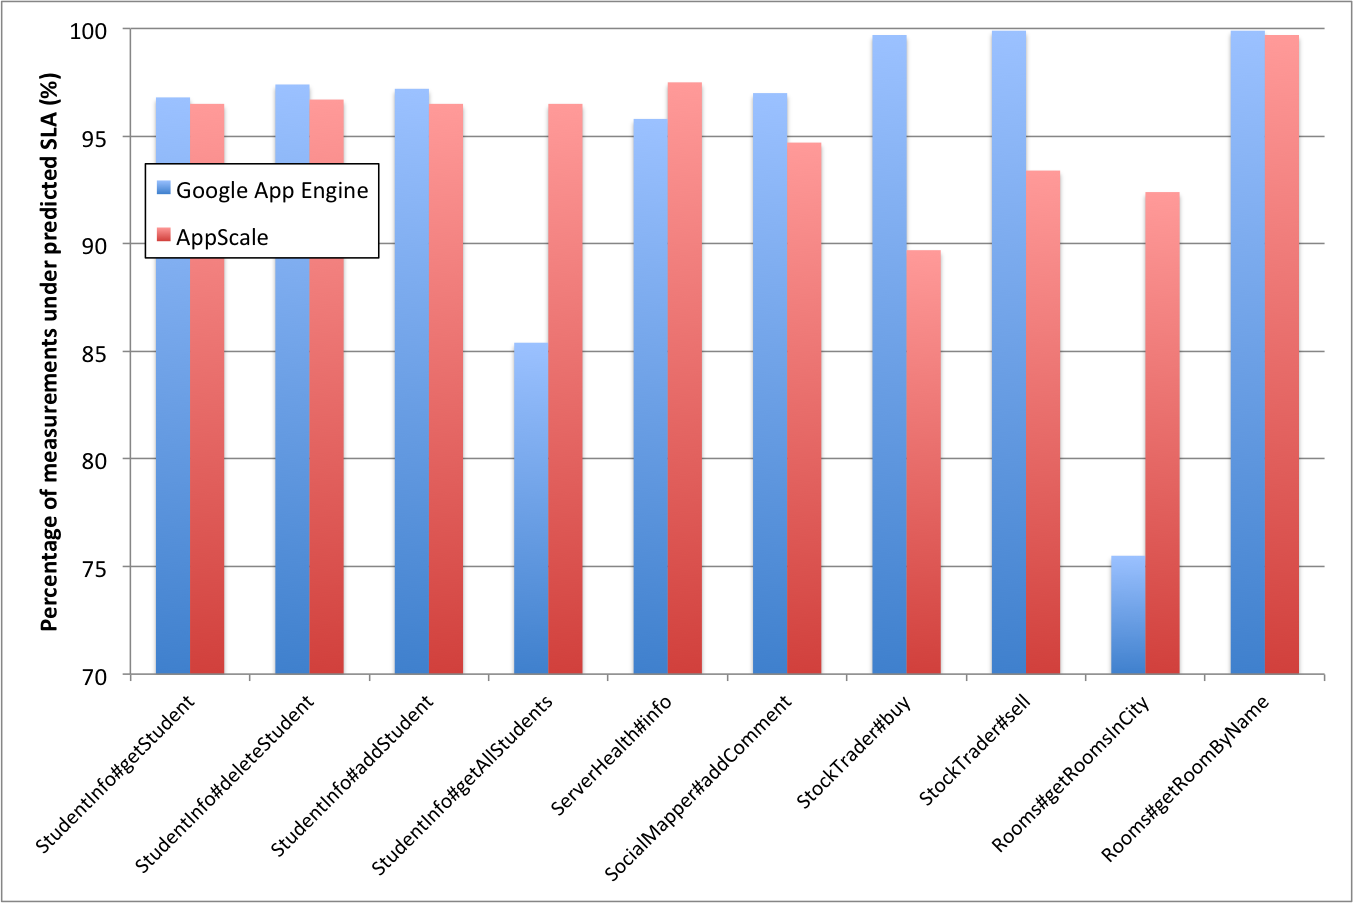
\includegraphics[scale=0.35]{simple_pred_accuracy_summary}
\caption{Cerebro correctness percentage resulting from the simple predictor (without QBETS).}
\label{fig:simple_pred_accuracy}
\vspace{-0.2in}
\end{figure}

For the simple predictor, Figure~\ref{fig:simple_pred_accuracy} shows lower 
correctness percentages compared to Figure~\ref{fig:accuracy_summary} for
QBETS (i.e. the simple predictor is less conservative).
However, in several cases the simple predictor falls well short of the target 
correctness of $95\%$ necessary for the SLA.  That is, it is unable to furnish
a prediction correctness that can be used as the basis of an
SLA in all of the test cases.
%This indicates that QBETS is a superior approach, albeit conservativeness,
%for making SLA predictions than simply
%calculating the percentiles on cloud SDK monitoring data.

To illustrate why the simple predictor fails to meet the desired correctness 
level, Figure~\ref{fig:get_rooms_in_city} shows the time series of observations, simple predictor forecasts,
and QBETS forecasts for the 
Rooms\#getRoomsInCity operation on Google App
Engine (the case in Figure~\ref{fig:simple_pred_accuracy} that shows 
lowest correctness percentage).
% the
%Rooms\#getRoomsInCity operation on Google App Engine (the case that shows
%lowest correctness fraction), 
%and compare its predicted SLAs
%against actual response times within a period of 1000 minutes. The resulting plot is shown in
%Figure~\ref{fig:get_rooms_in_city}. 
\begin{figure}
\centering
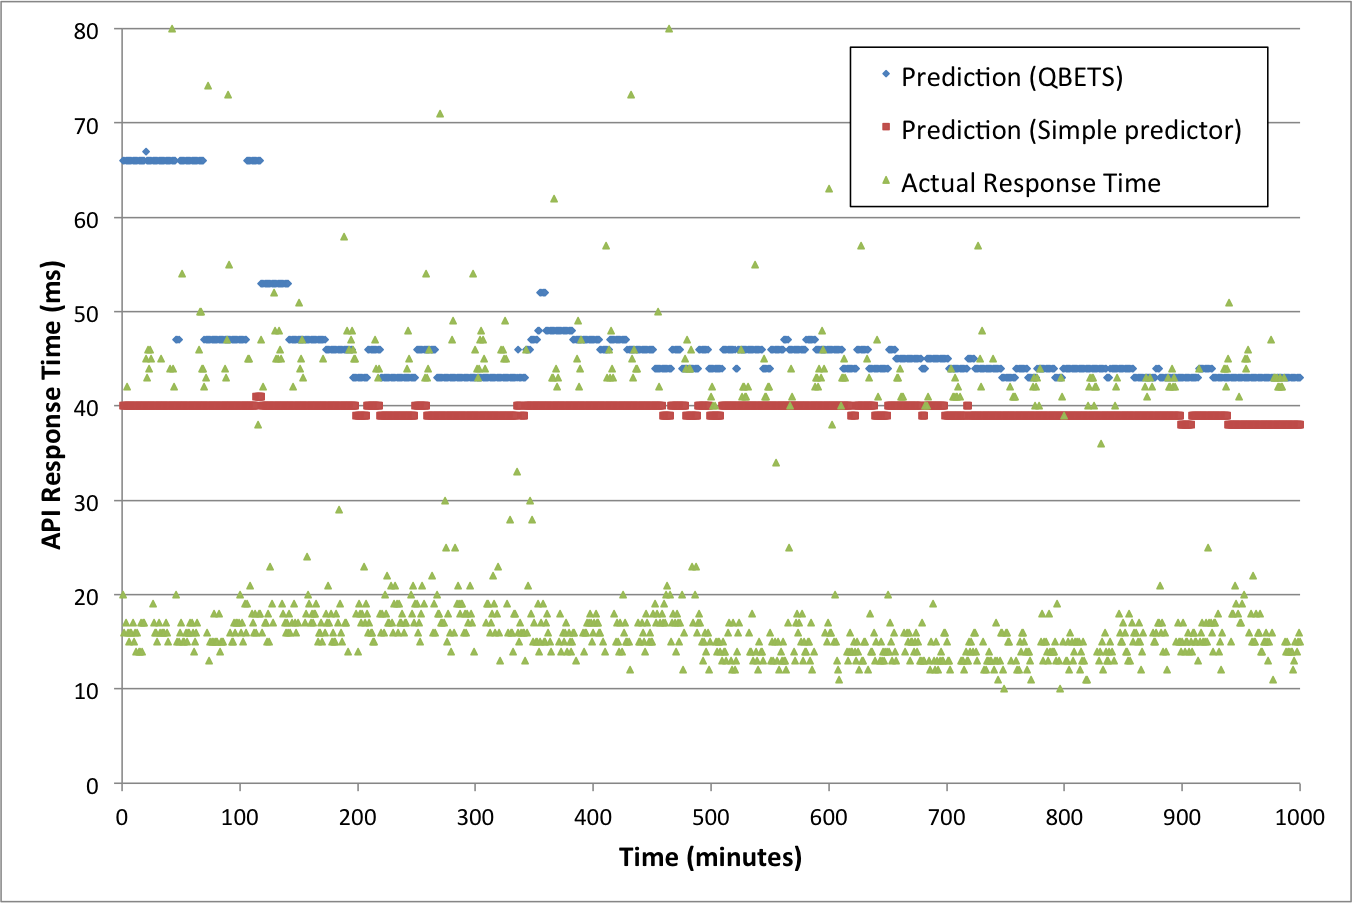
\includegraphics[scale=0.35]{get_rooms_in_city}
\caption{Comparison of predicted and actual response times of Rooms\#getRoomsInCity on Google App Engine.}
\label{fig:get_rooms_in_city}
\vspace{-0.2in}
\end{figure}

In this experiment, there are a significant number of response
time measurements that violate the SLA given by simple predictor (i.e. are
larger than the predicted percentile), but are below the corresponding QBETS
prediction made for the same observation.
Notice also that while QBETS is more conservative, (its predictions are
generally larger than those made by the simple predictor), in this case the
predictions are typically only $10\%$ larger.  That is, while the 
simple predictor shows the $95^{th}$ percentile to be approximately $40ms$,
the QBETS predictions vary between $42ms$ and $48ms$ (except at the beginning
where QBETS is ``learning'' the series).  This difference in prediction,
however, results in a large difference in correctness percentage.  For QBETS,
the correctness percentage is $97.3\%$ (Figure~\ref{fig:accuracy_summary}) compared to
$75.1\%$ for the simple predictor (Figure~\ref{fig:simple_pred_accuracy}).
%Thus, while QBETS is more conservative, it is able to make predictions that
%can be used as an SLA in this case (and in all of the cases we tested)
%where the simple predictor fails.

%As described in Subsection~\ref{sec:qbets},
%QBETS uses a form of supervised learning to determine each of its
%bound predictions.  
%As a result, the correctness percentage requires some number of state updates
%to converge to a stable value. We have observed that in the worst case, QBETS takes up to $200$ minutes to 
%achieve correctness percentage above $95\%$
%in Google App Engine.
%Alternatively, the longest time until QBETS has ``learned'' the series in
%AppScale is approximately $40$ minutes. Once this learning period has elapsed, QBETS
%generates predictions while consistently maintaining its correctness level above 95\%.

%\subsection{Learning Duration}
%\label{sec:learning}

%As described in Subsection~\ref{sec:qbets},
%QBETS uses a form of supervised learning internally to determine each of its
%bound predictions.  Each time a new prediction is presented, it updates its
%internal state with respect to autocorrelation and change-point detection.  As
%a result, the correctness percentage may require some number of state updates
%to converge to a stable value.

%Figure~\ref{fig:gae_accuracy} shows a running tabulation of
%correctness percentage for Cerebro
%predictions made in Google App Engine during the first 
%$1000$ minutes of operation (one prediction is generated each minute). 
%Similarly, in Figure~\ref{fig:as_accuracy} we show a running tabulation of
%correctness percentage for Cerebro
%predictions made in AppScale during the first 
%$1000$ minutes of operation (again, one prediction generated per minute). 

%\begin{figure}
%\centering
%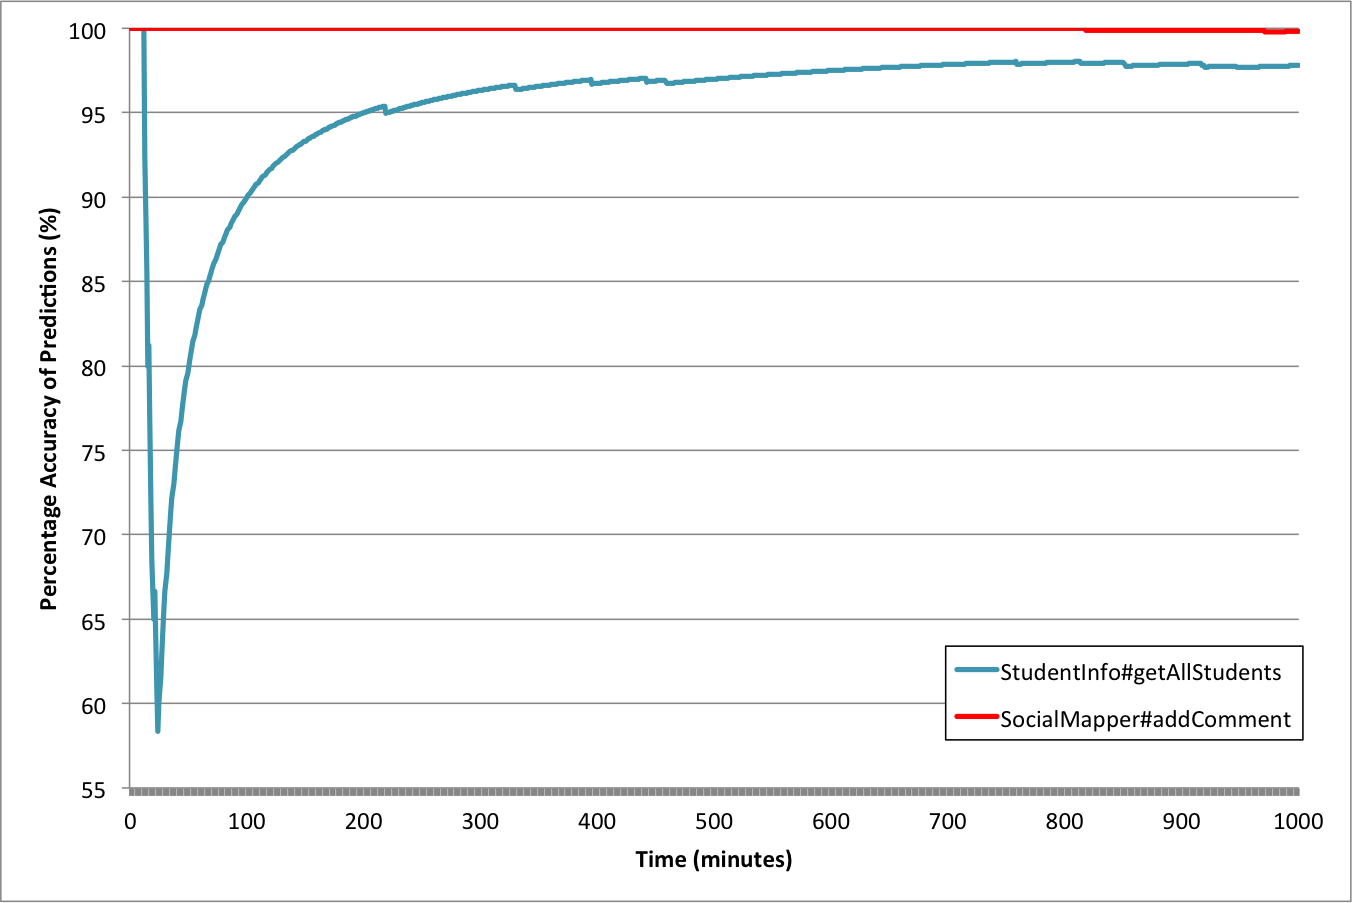
\includegraphics[scale=0.35]{gae_accuracy}
%\caption{Running tabulation of correctness percentage for predictions made on App Engine for a period
%of $1000$ minutes, one prediction per minute.}
%\label{fig:gae_accuracy}
%\vspace{-0.2in}
%\end{figure}

%\begin{figure}
%\centering
%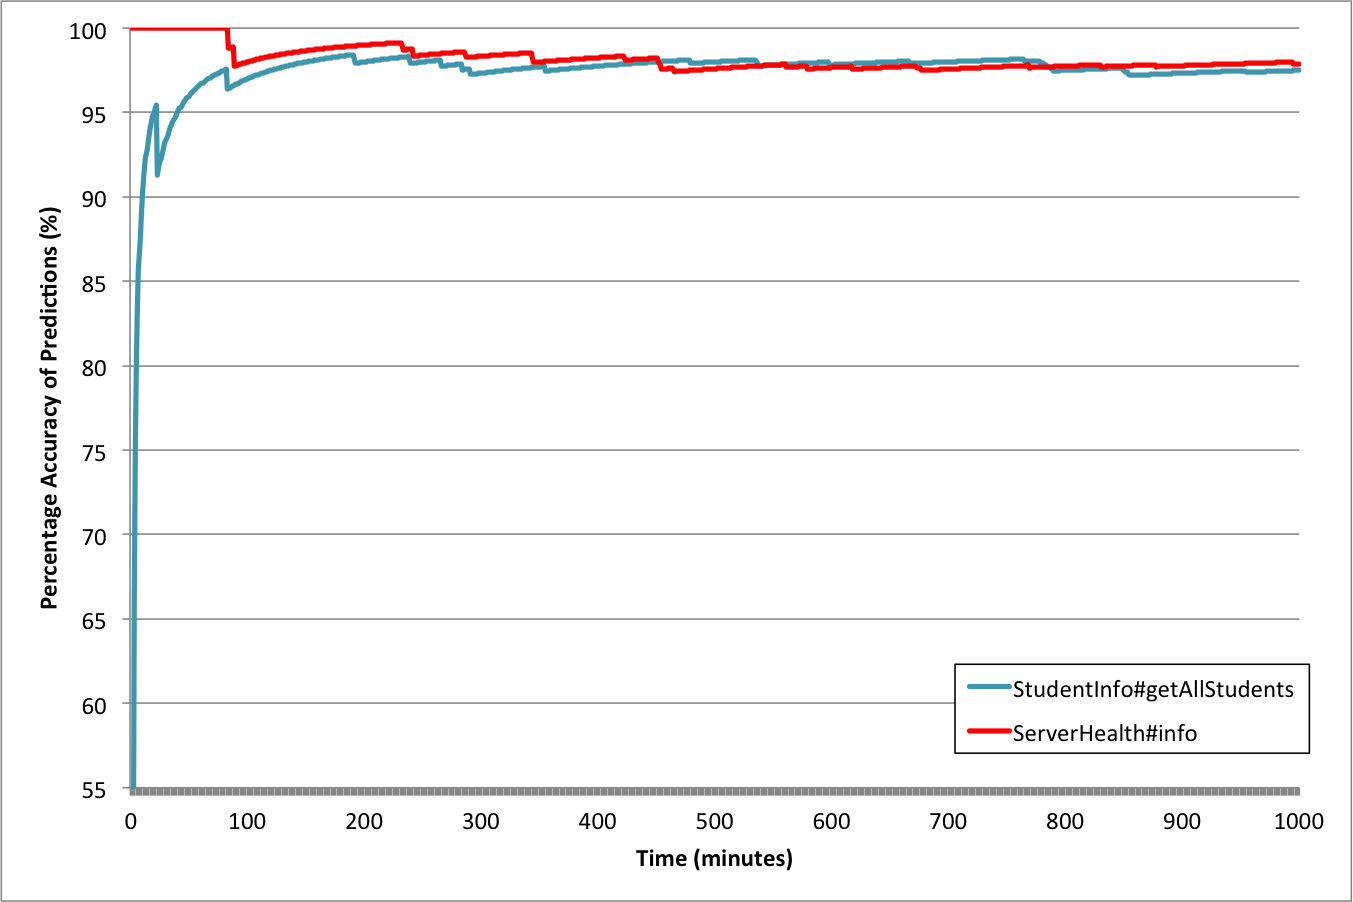
\includegraphics[scale=0.35]{as_accuracy}
%\caption{Running tabulation of correctness percentage for predictions made on AppScale for a period
%of $1000$ minutes, one prediction per minute.}
%\label{fig:as_accuracy}
%\vspace{-0.2in}
%\end{figure}

%For clarity we do not show results for all tested operations. Instead,
%we only show data for the operation that reaches stability in the shortest
%amount of time, and the operation that takes the longest to converge.
%Results for other operations fall between these two extremes.

%In the worst case, Cerebro takes up to $200$ minutes to 
%achieve correctness percentage above $95\%$
%in Google App Engine (for StudentInfo\#getAllStudents).
%Alternatively, the longest time until Cerebro has ``learned'' the series in
%AppScale is approximately $40$ minutes.

%Summarizing these results, 
%the learning time for Cerebro may be
%several hours (up to $200$ minutes in case of 
%Google App Engine), before it produces trustworthy and correct 
%SLA predictions.  The predictions made during this learning period are not
%necessarily incorrect.  It is just not possible to gauge their correctness
%quantitatively before the series has been learned.  We envision Cerebro as a
%continuous monitoring process in PaaS clouds for which ``startup time'' is not 
%an issue.


\vspace{-0.10in}
\section{Related Work}
\label{sec:related_work}
Our research builds upon advances in the areas of SOA governance and
service management. 
Guan et al introduced FASWSM~\cite{1607141} a web service management
framework for application servers. Wu et al introduced DART-Man~\cite{1504267} a web
service management system based on semantic web concepts. 
Our work is different from these past approaches and 
from recent API management solutions~\cite{wso2am,apigee}
in that EAGER targets policy \textit{enforcement} 
and we focus on doing so by extending extant
cloud platforms to provide an integrated and scalable governance
solution.

Lin et al proposed a service management system for clouds that monitors all
service interactions via special ``hooks'' that are connected to the
cloud-hosted services~\cite{5616981}. However, this system only supports run-time
service management and provides no support for deployment-time governance. 
Kikuchi and Aoki~\cite{6525502} proposed a technique
based on model checking to evaluate the operational vulnerabilities and fault
propagation patterns in cloud services. But this system provides no
active monitoring or enforcement functionality.

Other researchers have shown that policies can be
used to perform a wide range of governance tasks for SOA such as access
control~\cite{4279630}, fault diagnosis~\cite{6154236},
and management~\cite{Suleiman:2009:IUM:1564601.1564730}. We build
upon these past efforts and use policies to govern
RESTful web APIs deployed in cloud settings. 
Peng, Lui and Chen showed that
the major concerns associated with SOA governance 
involve retaining the high reliability of services, recording how many services
are available on the platform to serve, and making sure all the available 
services are operating within an acceptable service
level~\cite{4730489}. EAGER attempts to satisfy similar requirements for 
modern RESTful web APIs deployed in cloud environments. 
However, EAGER's Metadata Manager and ADP record and keep track of all deployed APIs 
in a comprehensive manner.  Moreover, EAGER's governance features 
``fail fast'' to detect violations immediately.

%API management has been a popular topic in industry recently, resulting
%in many API management solutions~\cite{wso2am,apigee}. These products facilitate
%API lifecycle management, traffic shaping, access control, monitoring and a variety of other
%important API-related functionality. However, these tools do not support deep integration with
%cloud environments in which many web applications and APIs are deployed.

%
%These API
%management products either run as stand-alone entities or are layered on top of existing clouds
%thus leading to many maintenance, reliability and integration issues. Also, the support provided by these
%tools to specify and enforce policies in a flexible manner is very limited. EAGER is complementary
%to such tools, providing very deep integration with PaaS clouds thereby facilitating API governance
%as a core cloud-native feature. Indeed, EAGER can embed and enhance some of these tools to
%obtain the required API governance support in the cloud. In fact, the EAGER prototype we have
%implemented makes extensive use of an existing open source API management product~\cite{wso2am}.


\vspace{-0.10in}
\section{Conclusions}
\label{sec:conclusions}
Web services and service oriented architecture encourage developers to create new applications by
composing existing services via their web APIs. But such integration of services makes it difficult to
reason about the performance and other non-functional properties of 
composite applications. To
facilitate such reasoning, web APIs should be exported for use
by applications with strong performance 
guarantees (SLAs).%, so that application developers are aware of 
%what to expect from the web APIs they consume. 

To this end,
we propose Cerebro, a system that predicts response time 
bounds for web APIs deployed in PaaS clouds. We
choose PaaS clouds as the target environment of our 
research due to their rapidly growing popularity as a technology
for hosting scalable web APIs, and their SDK-based, restricted 
application development model, 
which makes it easier to analyze PaaS applications statically.

Cerebro uses static analysis to extract the sequence of cloud SDK 
calls made by a given web API code combined with
historical performance measurements of cloud SDK calls to predict 
the response time of the web
API. 
%The historical performance data of cloud SDK 
%calls are gathered using a special monitoring agent
%executed in the PaaS cloud, that periodically benchmarks and records 
%cloud SDK performance, independent of deployed applications and web APIs.
It employs QBETS, a non-parametric time series analysis and 
forecasting method, to analyze
cloud SDK performance data, and predict bounds
on response time that can be used as statistical ``guarantees'' with
associated guarantee probabilities.
Cerebro is intended for use both during development and 
deployment phases of a web API, and 
precludes the need for continuous performance testing of the API code. 
Further, it does not interfere with the run-time operation (i.e. it requires
no application instrumentation at runtime) which makes it scalable.

We have implemented a prototype of Cerebro for Google App Engine public PaaS
and AppScale private PaaS
%We have subjected our
%prototype to a myriad of tests to study its efficacy in terms of
%correctness, tightness of predictions, and duration of prediction 
%validity.  
and evaluate it using a set of representative
and open source web applications developed by others.  
Our findings indicate that the prototype can determine response time levels
that correspond to specific target SLAs.  These predictions are also durable,
with average validity times varying between one and three days.

%And we use Cerebro to
%predict the 95th percentile of the API operation response time. 
%We find that:
%\vspace{-0.05in}
%\begin{itemize}
%\vspace{-0.05in}
%\item Cerebro achieves the desired correctness goal of 95\% for all the applications in both cloud environments.
%\vspace{-0.05in}
%\item Cerebro generates tight predictions (i.e.
%the predictions are similar to measured values) for most web APIs.  Because
%some operations and PaaS systems exhibit more variability in cloud SDK response
%time, 
%Cerebro must be conservative in some cases, and produce predictions that are less tight
%to meet its correctness guarantees.  
%\vspace{-0.05in}
%\item Cerebro requires a ``warm up'' period of up to 200 minutes to produce trustworthy predictions. Since PaaS systems are designed to run continuously, this is not an issue in practice. 
%\vspace{-0.05in}
%\item We can use a simple yet administratively useful model to identify when an 
%SLA becomes invalid to compute
%prediction validity durations for Cerebro.  The average duration of a valid
%Cerebro prediction is between 24 and 72 hours,
%and 95\% of the time this duration is at least 
%1.41 hours for App Engine and 1.95 hours for AppScale.
%\vspace{-0.05in}
%\end{itemize}
%\vspace{-0.05in}

In the current design, Cerebro's cloud SDK monitoring agent only monitors 
a predefined set of cloud SDK operations. In our future work we wish 
to explore the possibility of making this component more dynamic,
so that it automatically learns what operations to benchmark from the web APIs 
deployed in the cloud. This also includes learning the size and the form of the datasets
that cloud SDK invocations operate on, so that Cerebro can acquire more realistic
benchmarking data. Implementing these features might require non-invasively
instrumenting the deployed cloud applications. We also plan to investigate further how to better
handle data-dependent loops (iterative datastore reads) for different workloads. We are interested
in exploring the ways in which we can handle API codes with unpredictable execution patterns (e.g.
loops based on a random number), even though such cases are quite rare in the applications we
have looked at so far.
Further, we plan
to integrate Cerebro with EAGER, our API governance system 
and policy engine for PaaS clouds, so 
that PaaS administrators can enforce SLA-related policies on web APIs at deployment-time.
%Such a system will make it possible to prevent any API that 
%does not adhere to the organizational performance
%standards from being deployed in the production cloud environment.


%\appendix
%\section{Appendix Title}

%This is the text of the appendix, if you need one.

%\vspace{0.02in}
%\noindent
\acks
This work is funded in part by NSF (CNS-0905237, CNS-1218808, ACI-0751315) \& NIH
(1R01EB014877-01).

% We recommend abbrvnat bibliography style.
\bibliographystyle{abbrvnat}
\softraggedright
\bibliography{references}

% The bibliography should be embedded for final submission.

%\begin{thebibliography}{}
%\softraggedright

%\bibitem[Smith et~al.(2009)Smith, Jones]{smith02}
%P. Q. Smith, and X. Y. Jones. ...reference text...

%\end{thebibliography}


\end{document}

%                       Revision History
%                       -------- -------
%  Date         Person  Ver.    Change
%  ----         ------  ----    ------

%  2013.06.29   TU      0.1--4  comments on permission/copyright notices

